\section{Defense strategy}
\begin{frame}
    \frametitle{Initial idea}
    We can 'concentrate' the mark in parts that are better at hiding it (like wavelet embedding)
\end{frame}

\subsection{Embedding}
\begin{frame}
    \frametitle{Embedding steps}
    Given a mark of size $N$:
    \begin{enumerate}
        \item<1-> Divide the image into M sub-blocks
        \item<2-> Find $M$ blocks with the highest variance ("candidate blocks")
        \item<3-> Embed $N/M$ parts of the mark into each candidate block, where each new coefficient of the watermarked image is defined as: %$1 + (\alpha \cdot \text{mark}[\text{mark_index}])$ 
              \[x_{ij}^* = x_{ij}[1 + (\alpha m_i)]\]
    \end{enumerate}

    \begin{figure}[h]
        \centering
        \subfloat{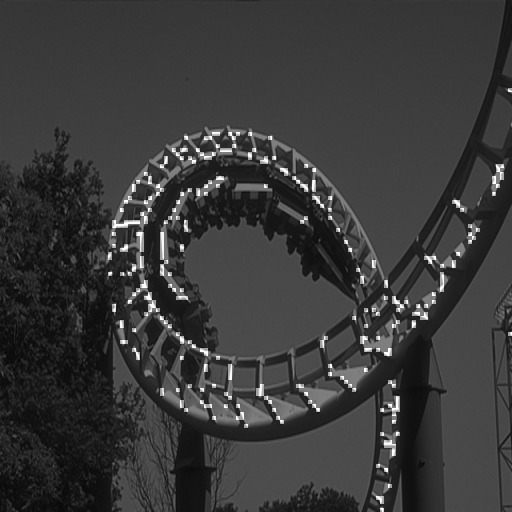
\includegraphics[width=.25\textwidth]{../drawable/rollercoaster-examples/rollercoaster_4_def.jpg}} \quad
        \subfloat{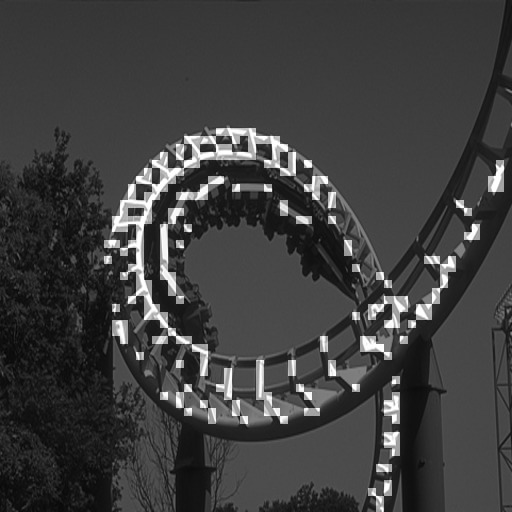
\includegraphics[width=.25\textwidth]{../drawable/rollercoaster-examples/rollercoaster_8_def.jpg}} \quad
        \subfloat{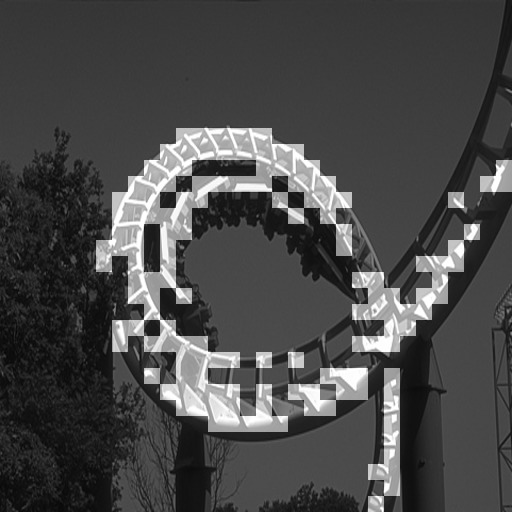
\includegraphics[width=.25\textwidth]{../drawable/rollercoaster-examples/rollercoaster_16_def.jpg}}
        \caption{Example of candidate blocks in the 'rollercoaster' image, with different block sizes}
        \label{fig:blocks_rollecoaster}
    \end{figure}
\end{frame}

\begin{frame}
    \frametitle{The \texttt{texture\_areas} function}
    The \texttt{texture\_areas} function is called by both the embedding and detection functions and provides them with a list of ordered blocks, in which the watermark will be inserted or detected.

    \medskip

    \onslide<2->{
        The function computes the variance of the image and then divides it into $n \times n$ blocks. Each block's variance is computed and then tested against the image's. If it is greater, then the block is added to the list.
    }

    \medskip
    \onslide<3->{
        Since some images may have an unsatisfactory number of high-variance blocks (e.g. very flat images with small contrast areas), the function will recursively call itself, lowering the variance theshold each time until either it runs out of iterations or finds enough blocks.
    }
\end{frame}

\begin{frame}
    \frametitle{The \texttt{texture\_areas} function}
    The function uses a threshold based on the \texttt{sqrt} of the variance in order to decide when to stop searching for blocks. Its choice is purely experimental: we tried with different indicators but found the square root the most flexible.

    \medskip

    \onslide<2->{
        Its great flexibility means it can easily be adapted to the situation by fastening or slowing the search, changing the block size, and so on.
    }

    \medskip

    \onslide<3->{
        Finally, found blocks are sorted by variance and sent back to the caller.
    }
\end{frame}

\begin{frame}
    \frametitle{The \texttt{texture\_areas} function}

    In short, the parameters are:
    \begin{itemize}
        \item<1-> \texttt{block\_size}: the size of the searched blocks.
        \item<2-> \texttt{coeff}: a float that divides the variance (and since it's usually $> 0$, it reduces it) when the algorithm decides whether or not to choose a block
        \item<3-> \texttt{max\_iteration}: maximum recursion depth
        \item<4-> \texttt{var\_multiplier, coeff\_step}: at the recursion point, the algorithm does the following:

              \texttt{if len(result) < var\_multiplier * math.sqrt(image\_variance):}\\
              \texttt{\hphantom{hhhhh}texture\_areas(image, block\_size,}\\
                  \texttt{\hphantom{hhhhhhhhhhhhhhhhhhh}coeff / var\_multiplier,} \texttt{\hphantom{hhhhhhhhhhhhhhhhhhh}result, it=it + 1)}

    \end{itemize}
\end{frame}

\begin{frame}
    \frametitle{The \texttt{texture\_areas} function, changing parameters}
    \begin{figure}[h]
        \centering
        \subfloat{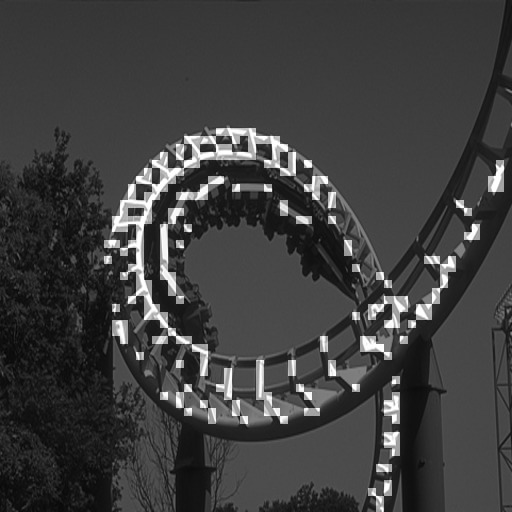
\includegraphics[width=.25\textwidth]{../drawable/rollercoaster-examples/rollercoaster_8_def.jpg}} \quad
        \subfloat{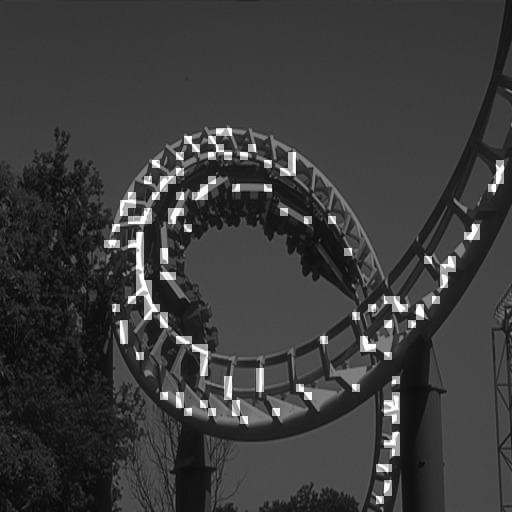
\includegraphics[width=.25\textwidth]{../drawable/rollercoaster-examples/rollercoaster_8_2coeff_1var.jpg}} \quad
        \subfloat{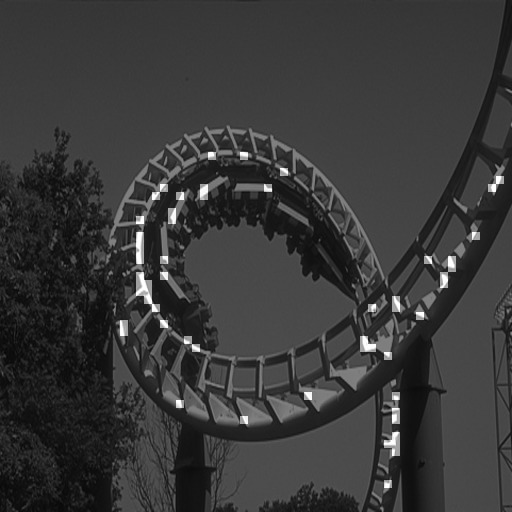
\includegraphics[width=.25\textwidth]{../drawable/rollercoaster-examples/rollercoaster_8_4coeff_1var.jpg}}
        \caption{Example of candidate blocks in the 'rollercoaster' image, when the $coeff$ coefficient is changed}
        \label{fig:blocks_rollecoaster_2}
    \end{figure}
\end{frame}

\begin{frame}
    \frametitle{The \texttt{texture\_areas} function, changing parameters}
    \begin{figure}[h]
        \centering
        \subfloat{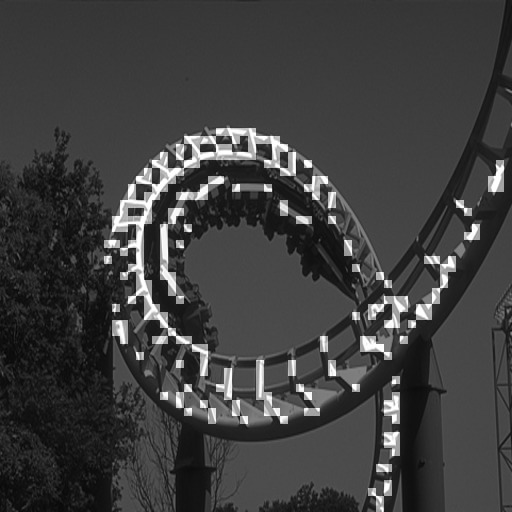
\includegraphics[width=.25\textwidth]{../drawable/rollercoaster-examples/rollercoaster_8_def.jpg}} \quad
        \subfloat{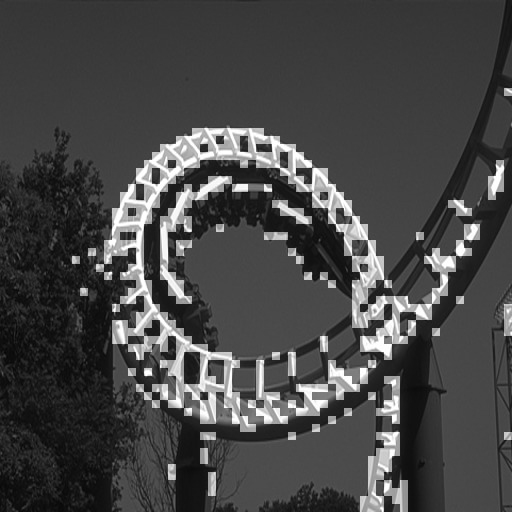
\includegraphics[width=.25\textwidth]{../drawable/rollercoaster-examples/rollercoaster_8_40var.jpg}}
        \caption{Example of candidate blocks in the 'rollercoaster' image, when the $var_coeff$ coefficient is changed}
        \label{fig:blocks_rollecoaster_3}
    \end{figure}
\end{frame}

\subsection{Detection}

\begin{frame}
    \frametitle{Detection steps}
    \begin{enumerate}
        \item<1-> Find candidate blocks using the original image  $\Rightarrow$ this is possible because detection is non-blind.
        \item<2-> Extract mark from candidate blocks
        \item<3-> Reassemble mark
              \begin{figure}[h]
                  \centering
                  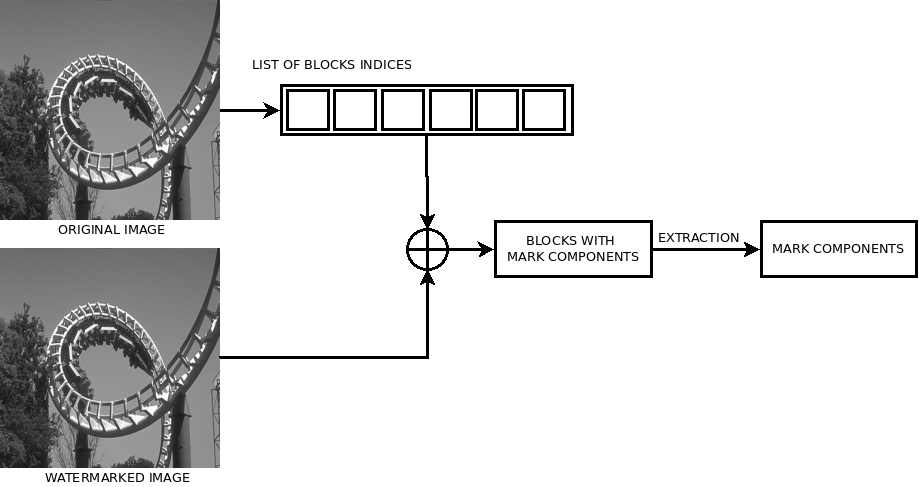
\includegraphics[width=0.85\textwidth]{../drawable/extracting-blocks.png}
                  \label{fig:mark_extraction}
              \end{figure}
    \end{enumerate}
\end{frame}

\begin{frame}
    \frametitle{Strength and weaknesses}
    Strengths:

    \begin{itemize}
        \item Strong parametrization and flexibility
        \item Fast (statistically insignificant slowdowns compared to standard SS watermarking)
        \item Easily extensible by changing employed metrics
        \item At lower $\alpha$, very high WPSNR and undetectable by the naked eye
    \end{itemize}
    \onslide<2->{
        Weaknesses:

        \begin{itemize}
            \item Extremely dependent on the image features
            \item Embedded blocks locations are deterministic and predictable to the attacker
            \item \textbf{Underflow/overflow problems} when converting from DCT domain to pixel domain
        \end{itemize}
    }
\end{frame}

\begin{frame}
    \frametitle{One-attack test results}

    \only<1>{
        \begin{figure}
            \centering
            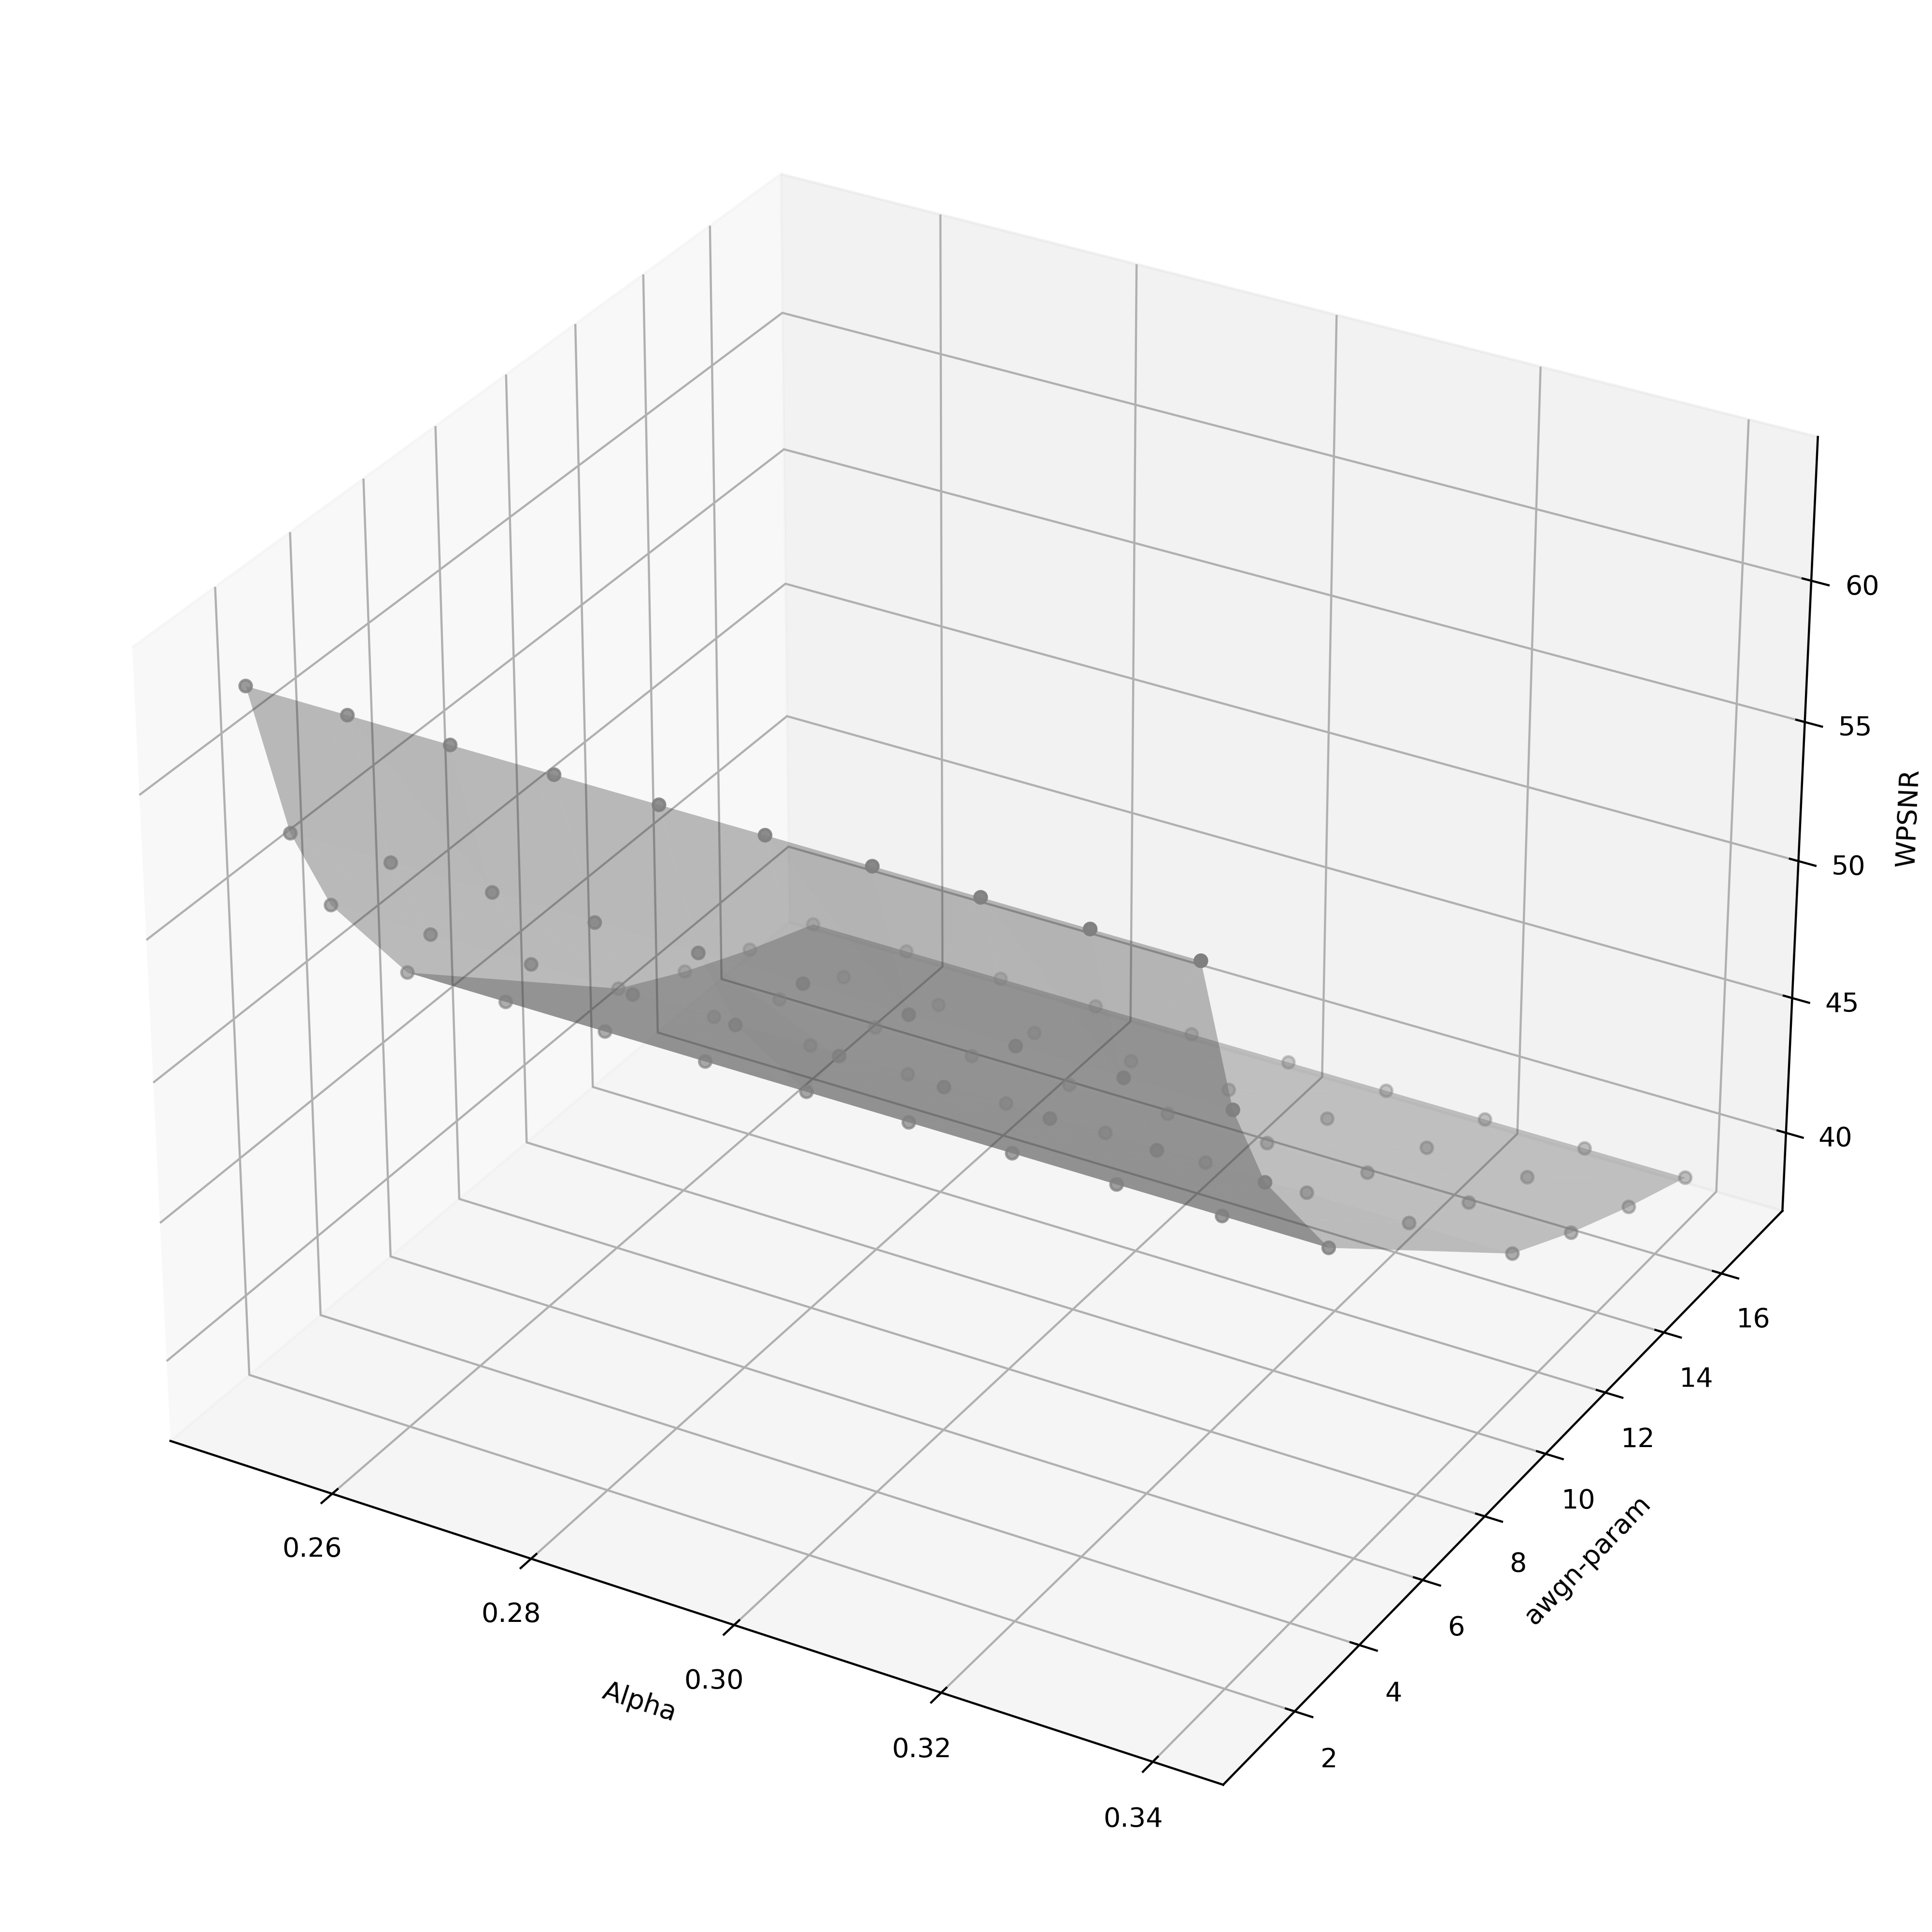
\includegraphics[width=0.5\textwidth]{../drawable/classic-attacks-plots/awgn-alpha.png}
            \caption{Plot of $\alpha$, WPSNR and AWGN attacks (random seed). Red dots are successful attacks.}
        \end{figure}
    }

    \only<2>{
        \begin{figure}
            \centering
            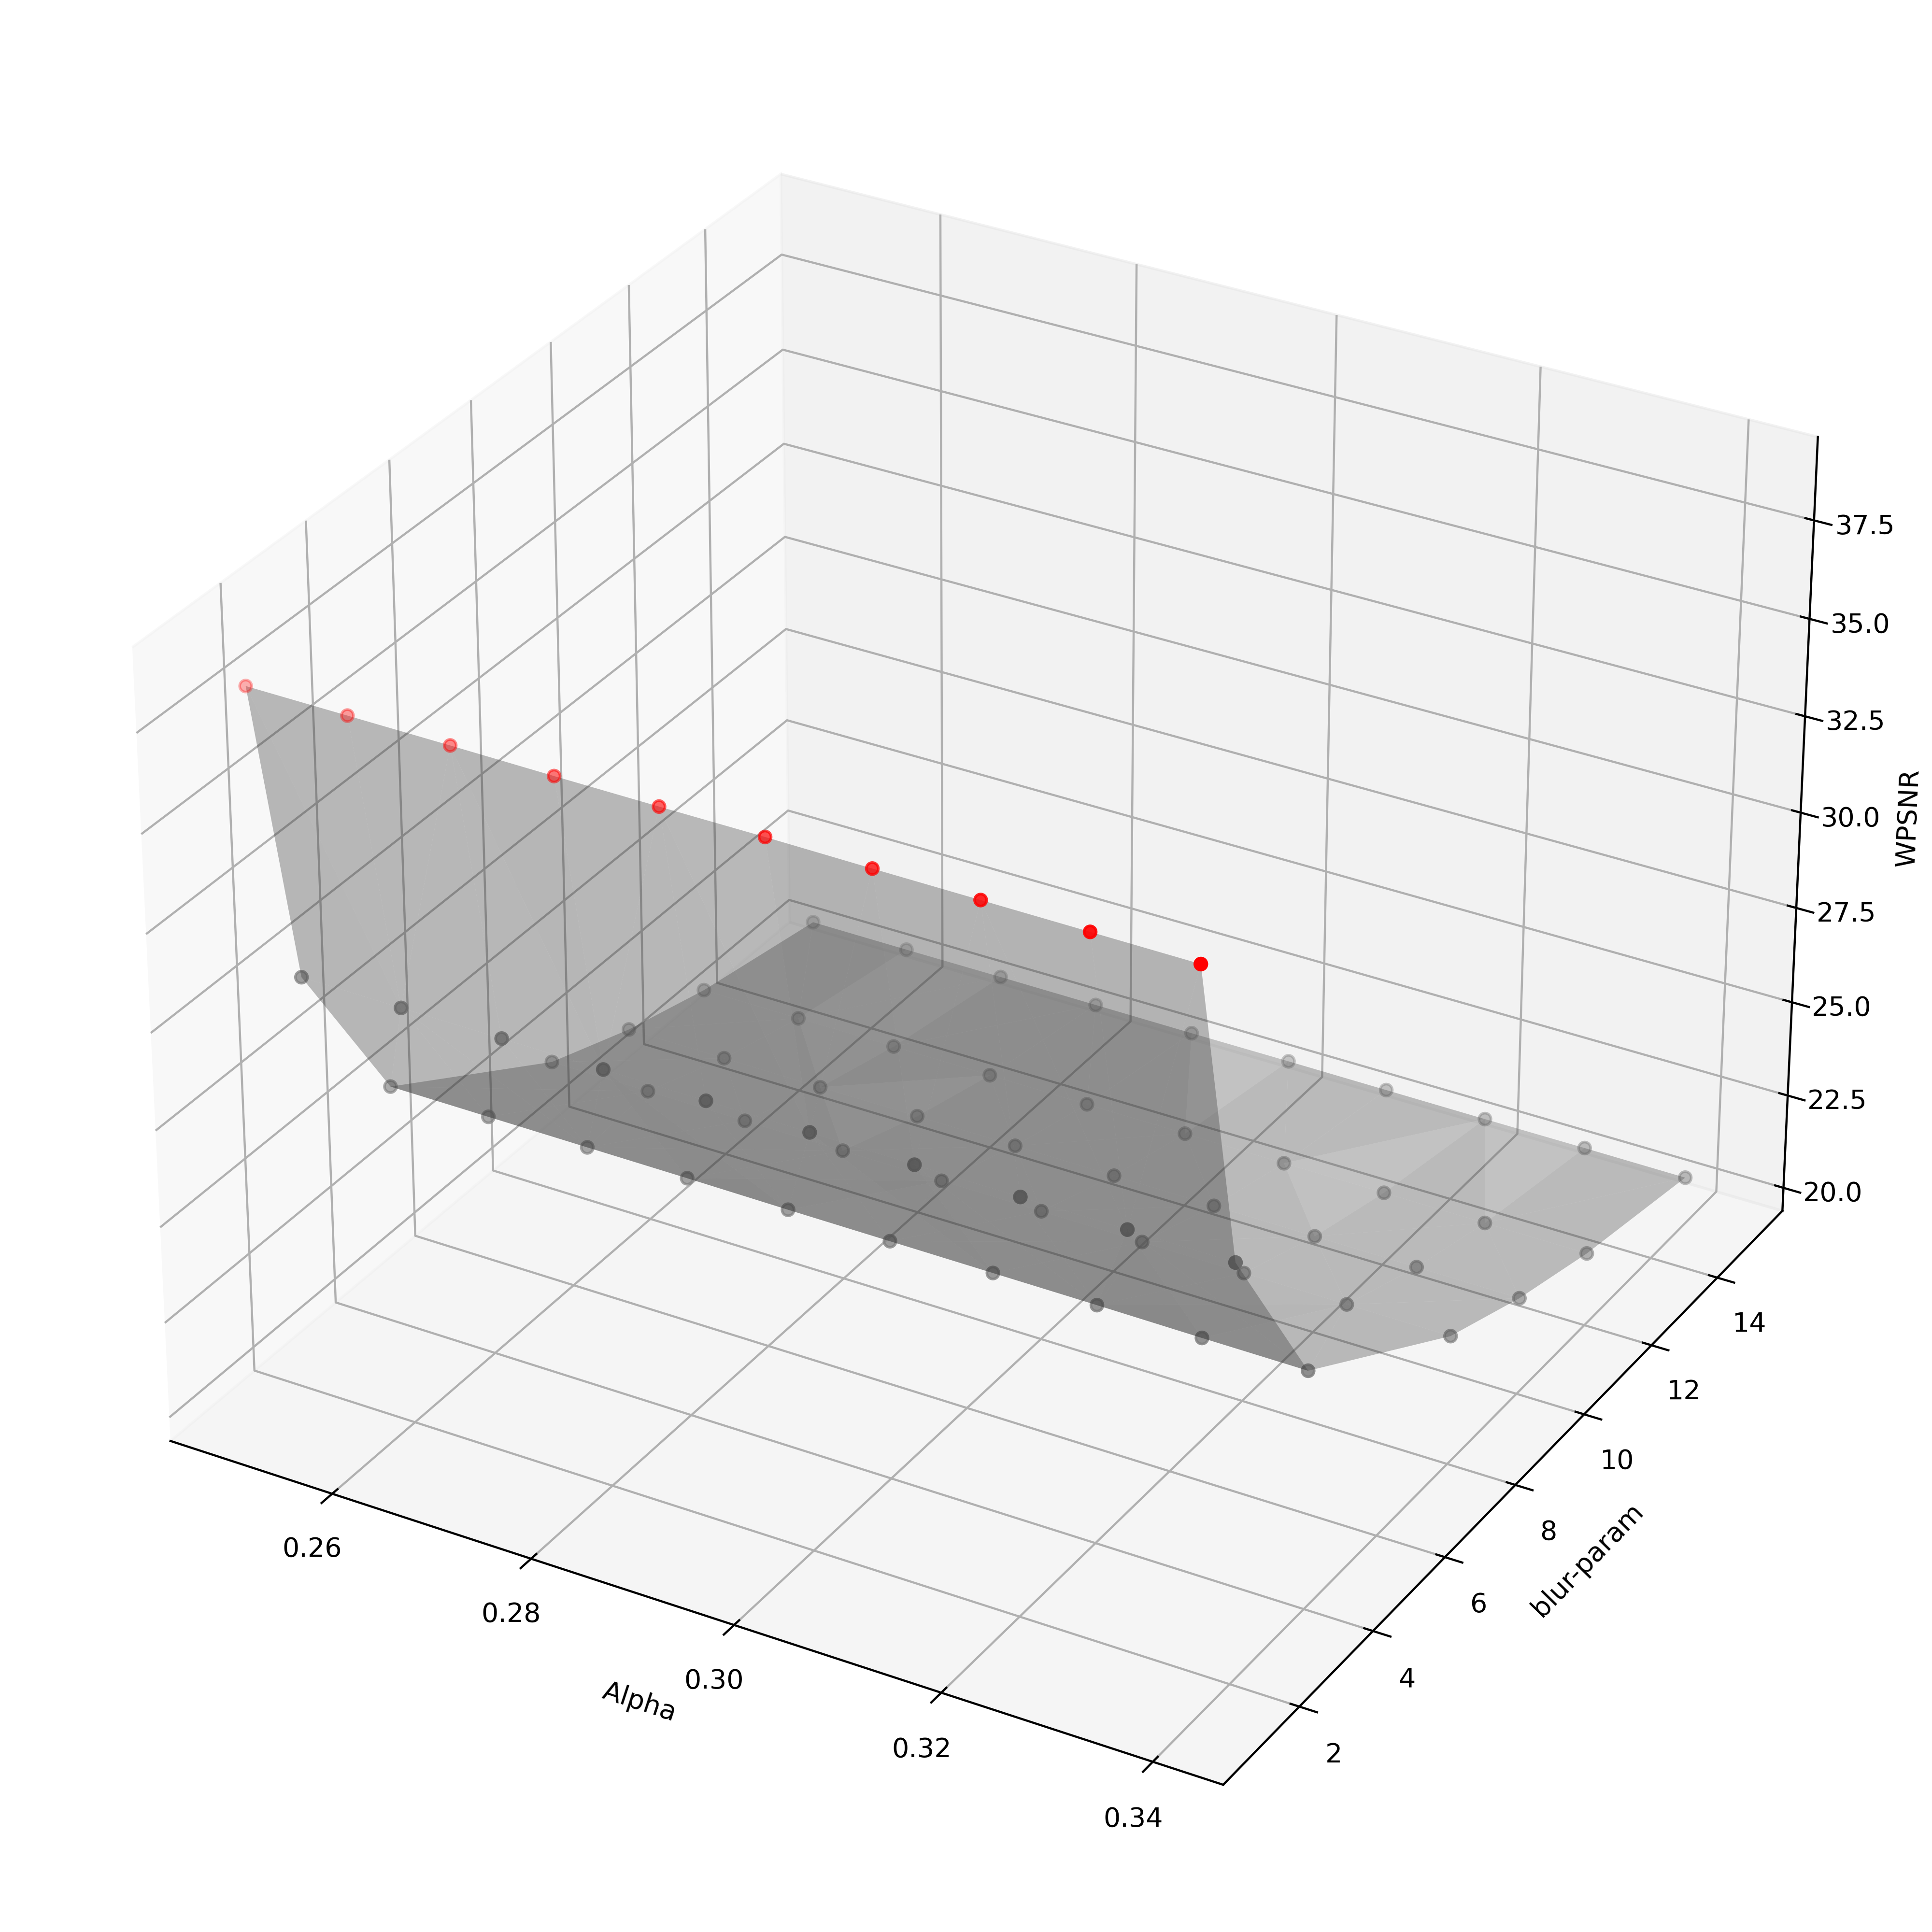
\includegraphics[width=0.5\textwidth]{../drawable/classic-attacks-plots/blur-alpha.png}
            \caption{Plot of $\alpha$, WPSNR and blur attacks. Red dots are successful attacks.}
        \end{figure}
    }

    \only<3>{
        \begin{figure}
            \centering
            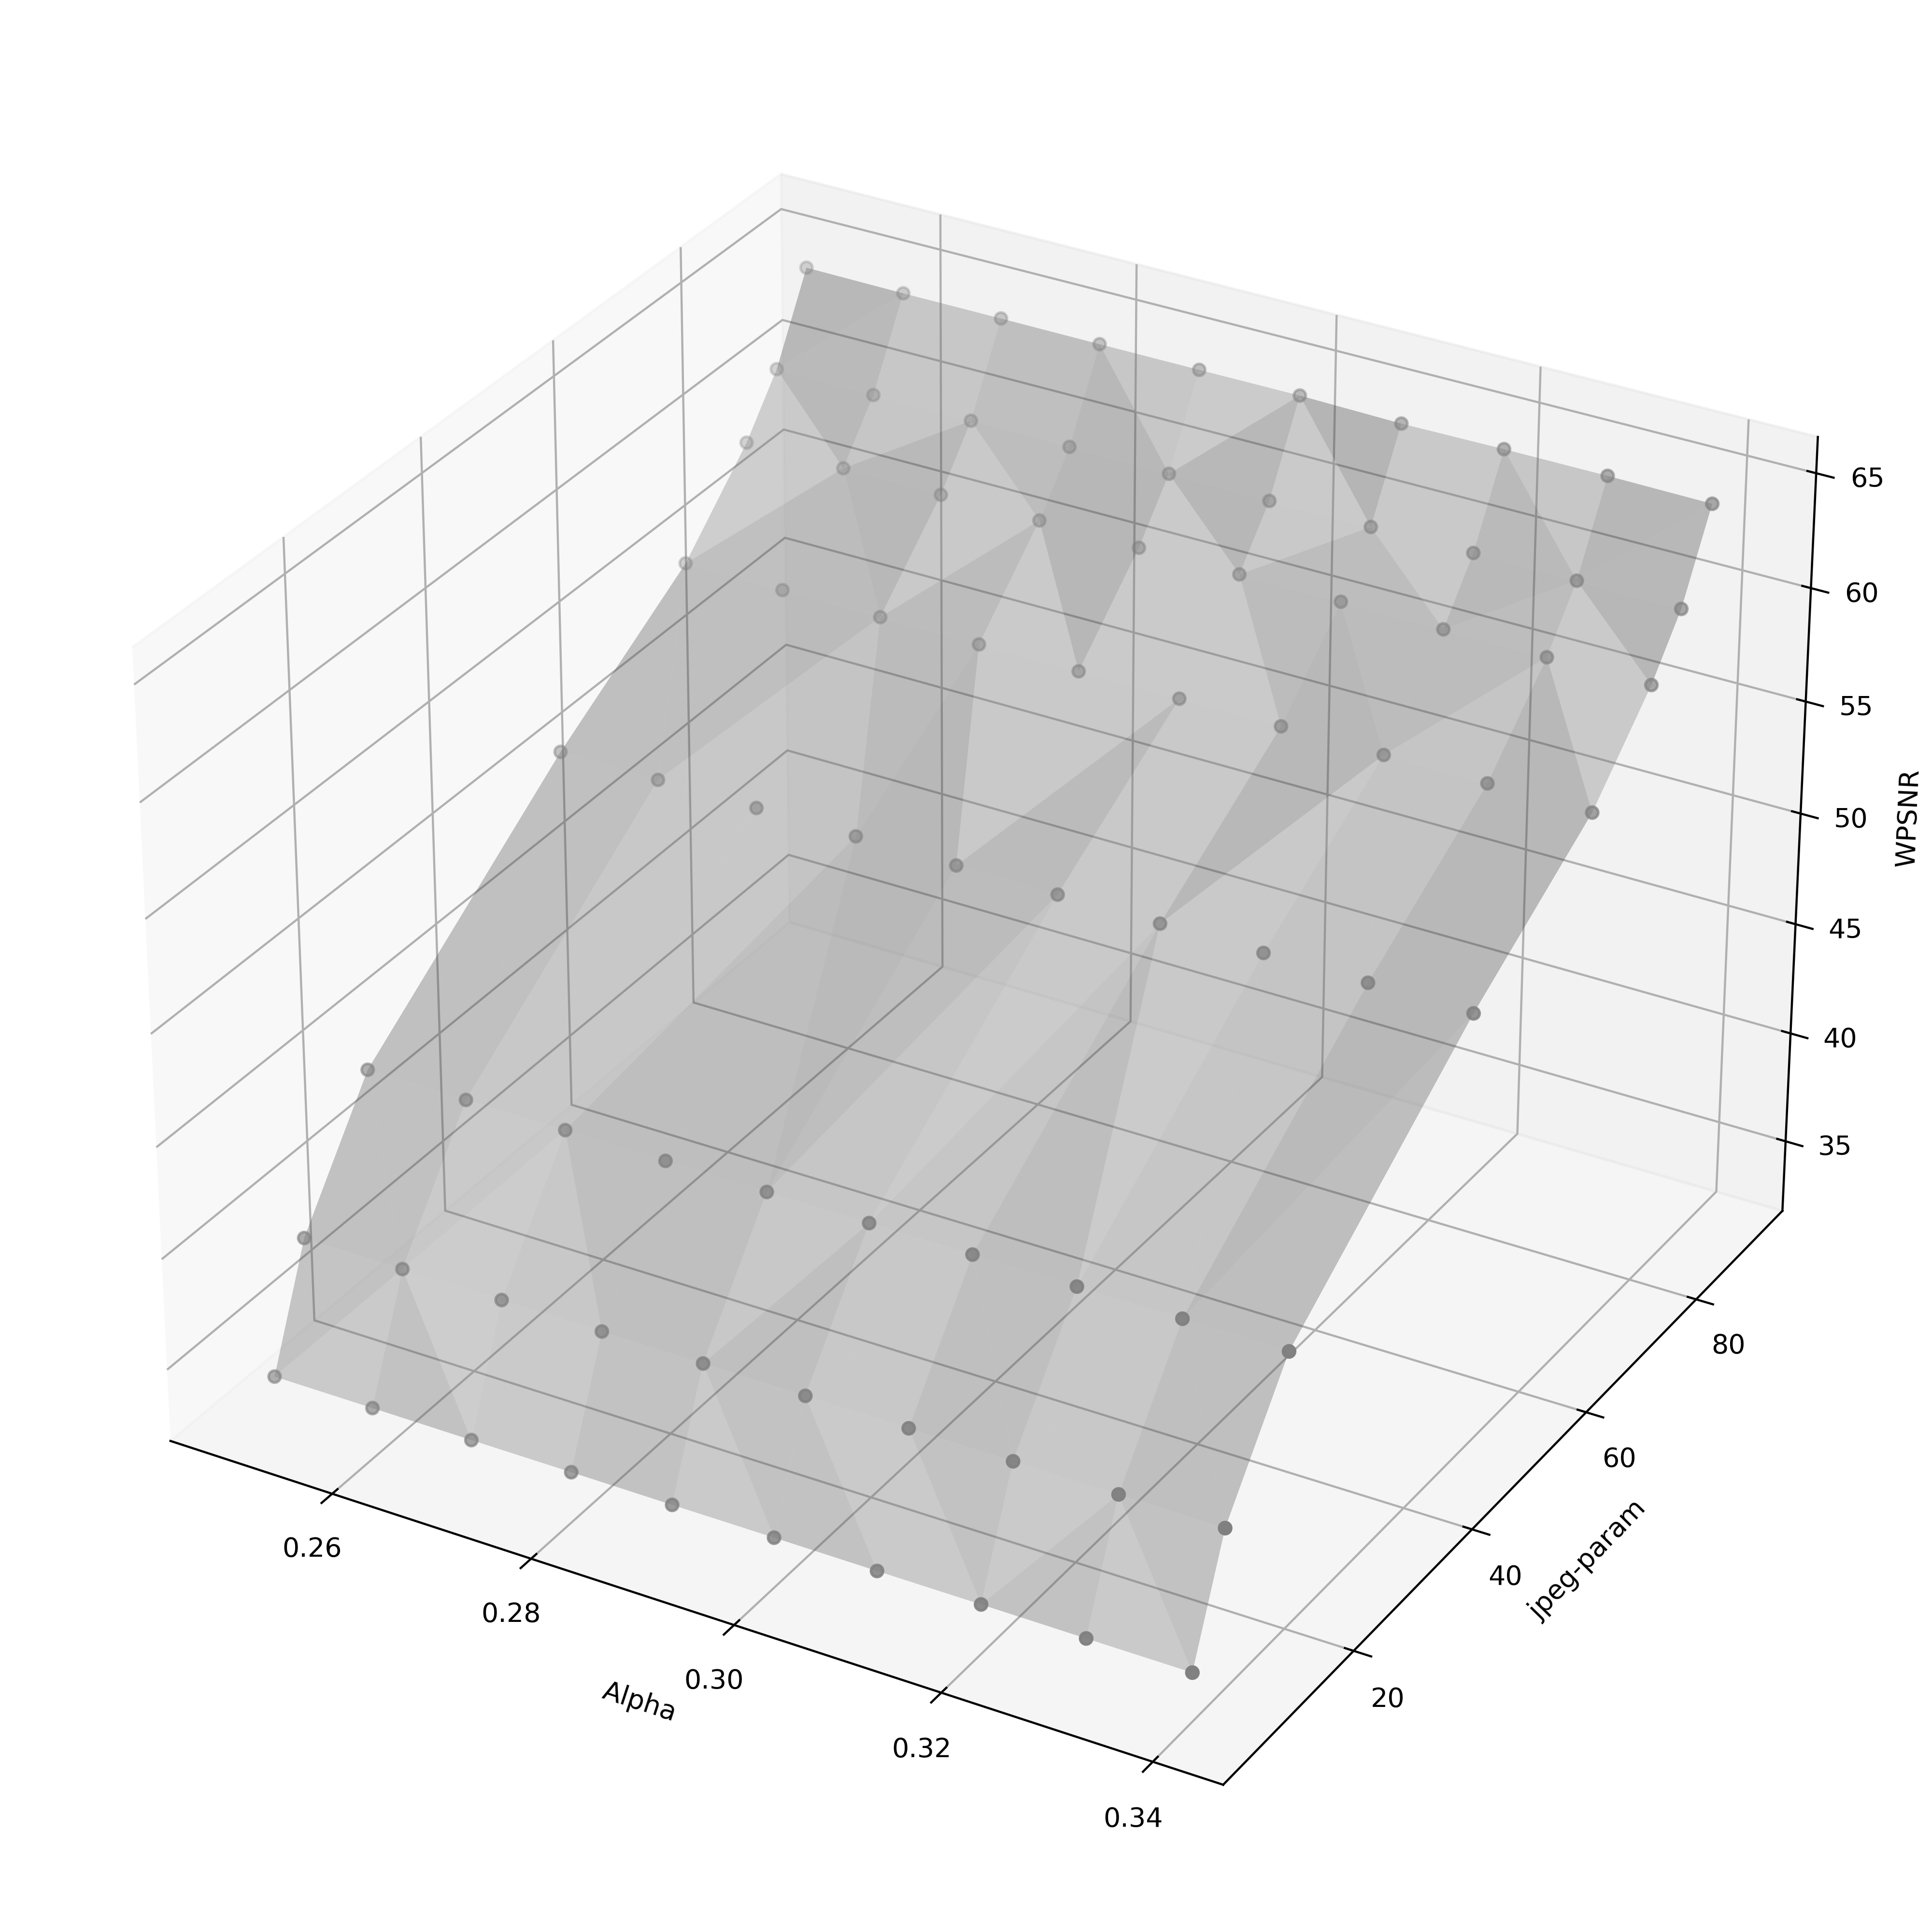
\includegraphics[width=0.5\textwidth]{../drawable/classic-attacks-plots/jpeg-alpha.png}
            \caption{Plot of $\alpha$, WPSNR and JPEG attacks. Red dots are successful attacks.}
        \end{figure}
    }

    \only<4>{
        \begin{figure}
            \centering
            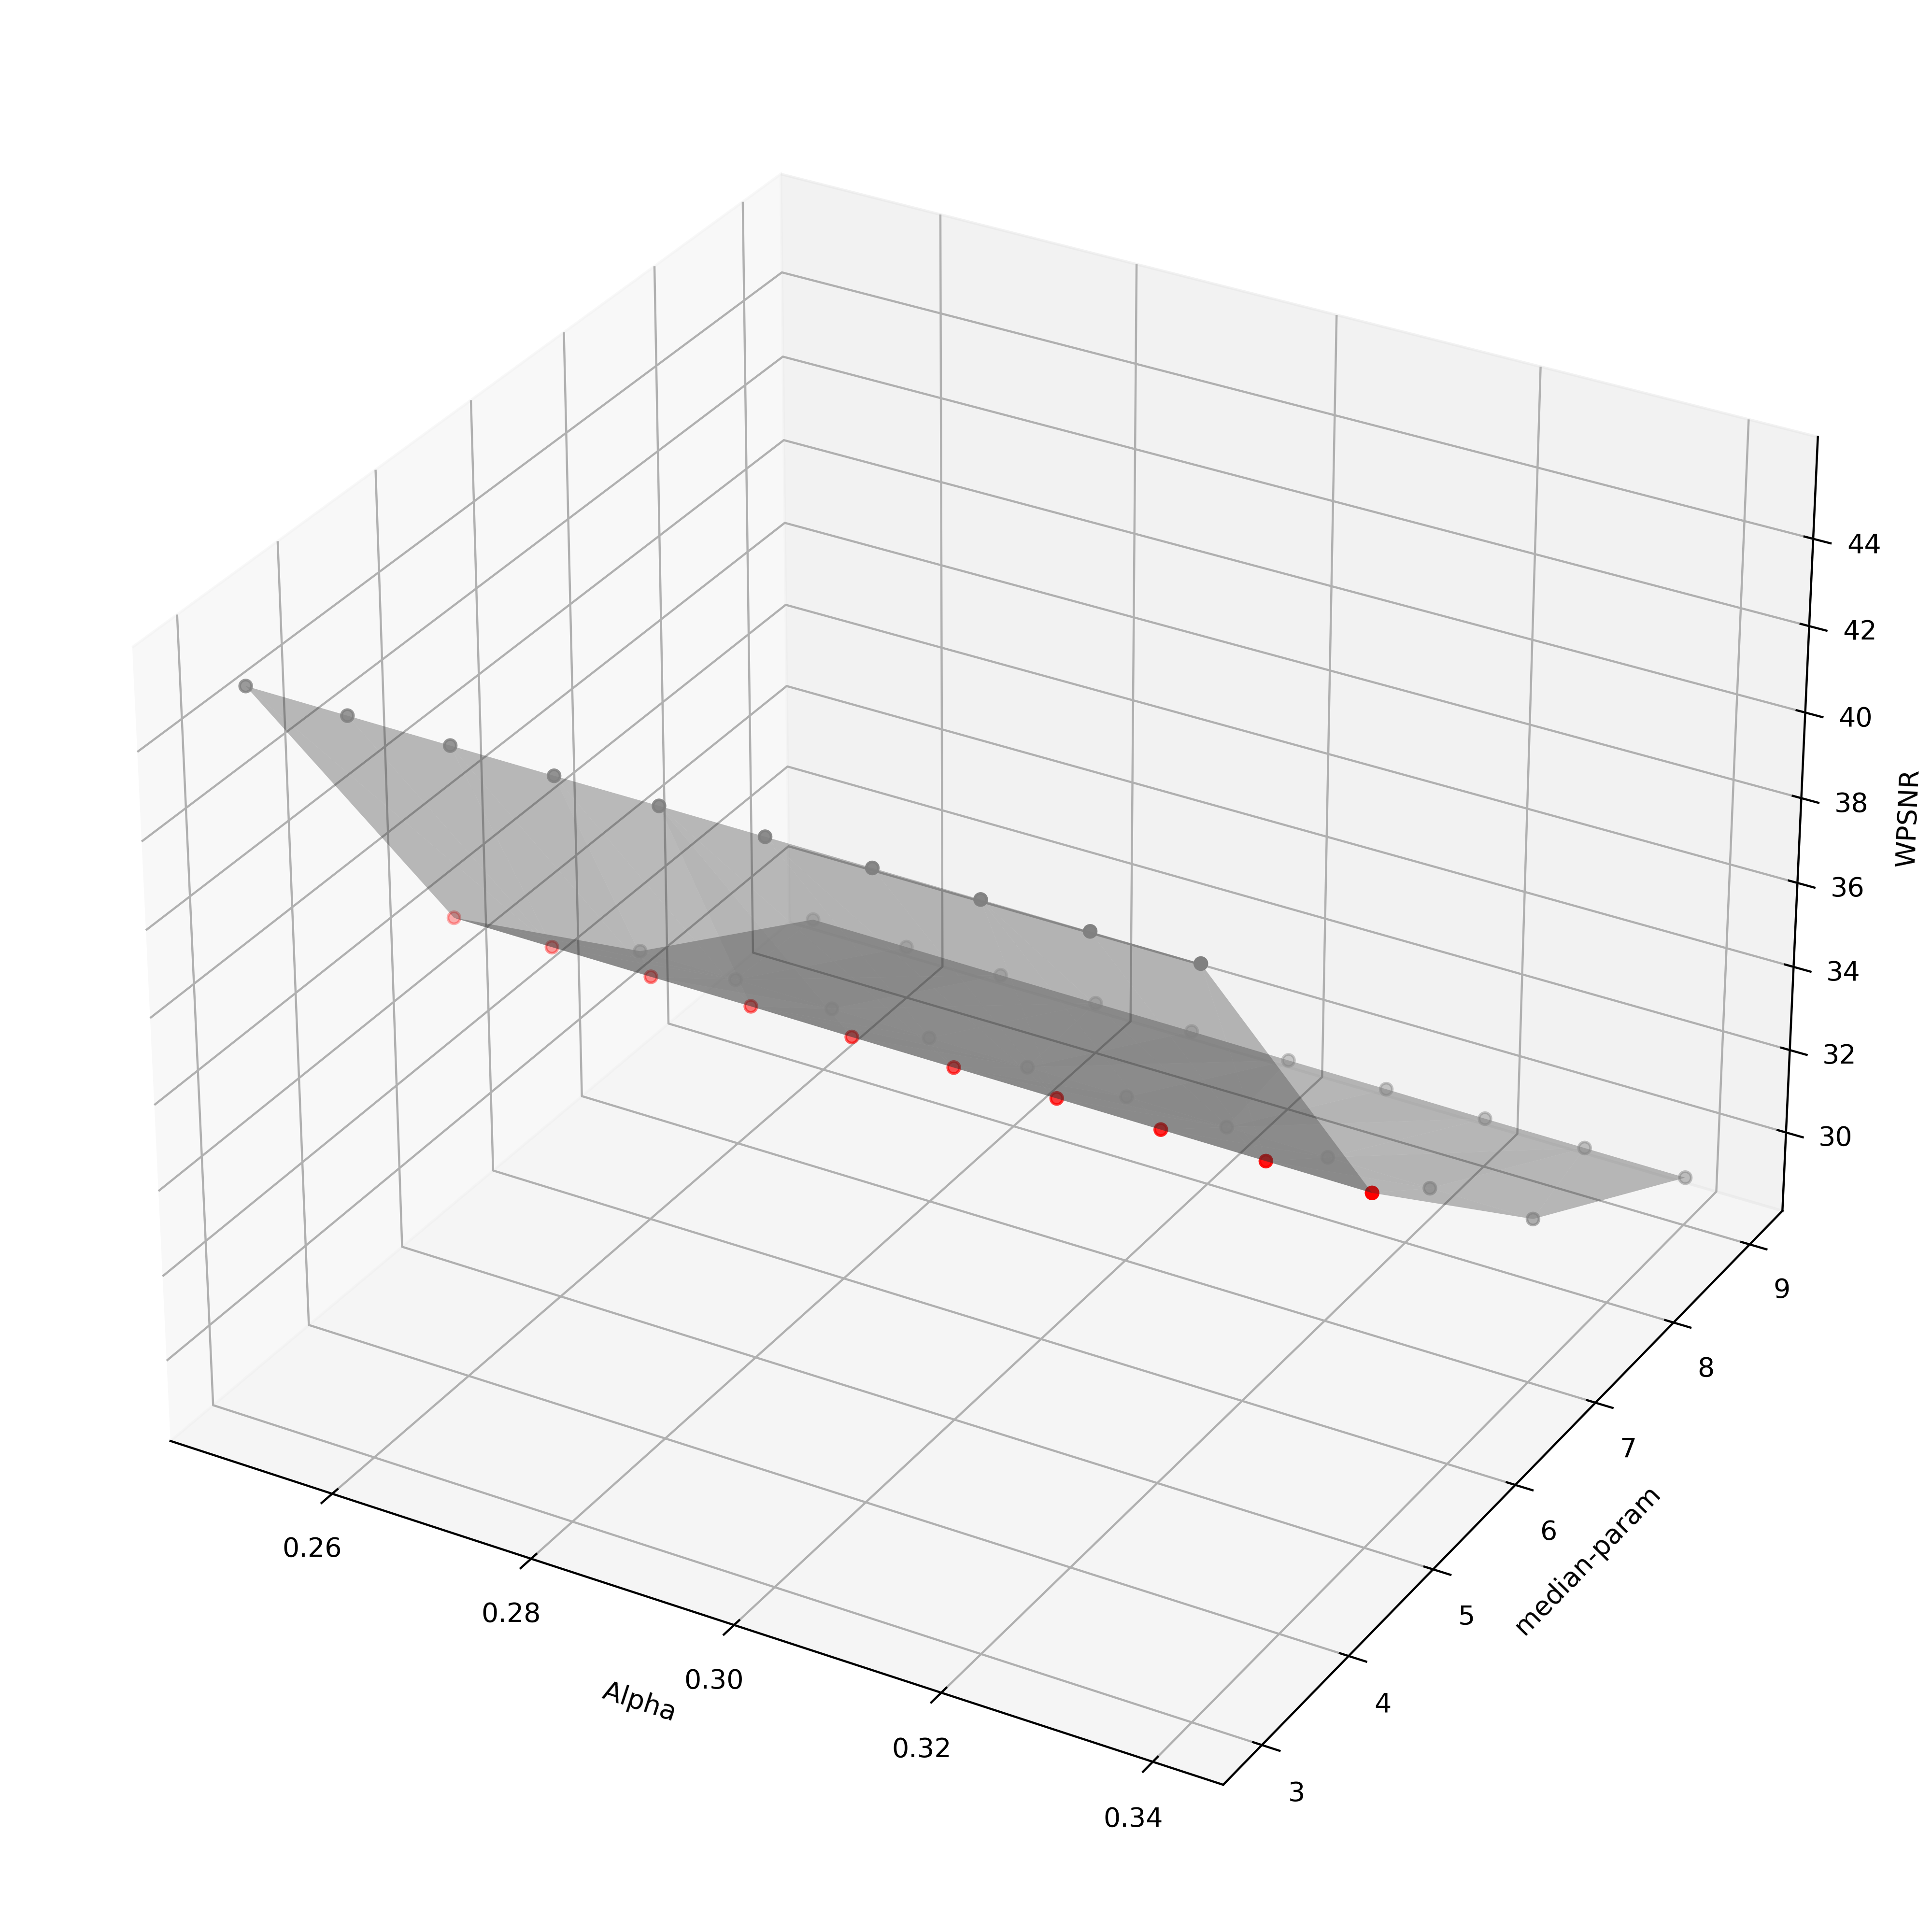
\includegraphics[width=0.5\textwidth]{../drawable/classic-attacks-plots/median-alpha.png}
            \caption{Plot of $\alpha$, WPSNR and median attacks (square sliding window). Red dots are successful attacks.}
        \end{figure}
    }

    \only<5>{
        \begin{figure}
            \centering
            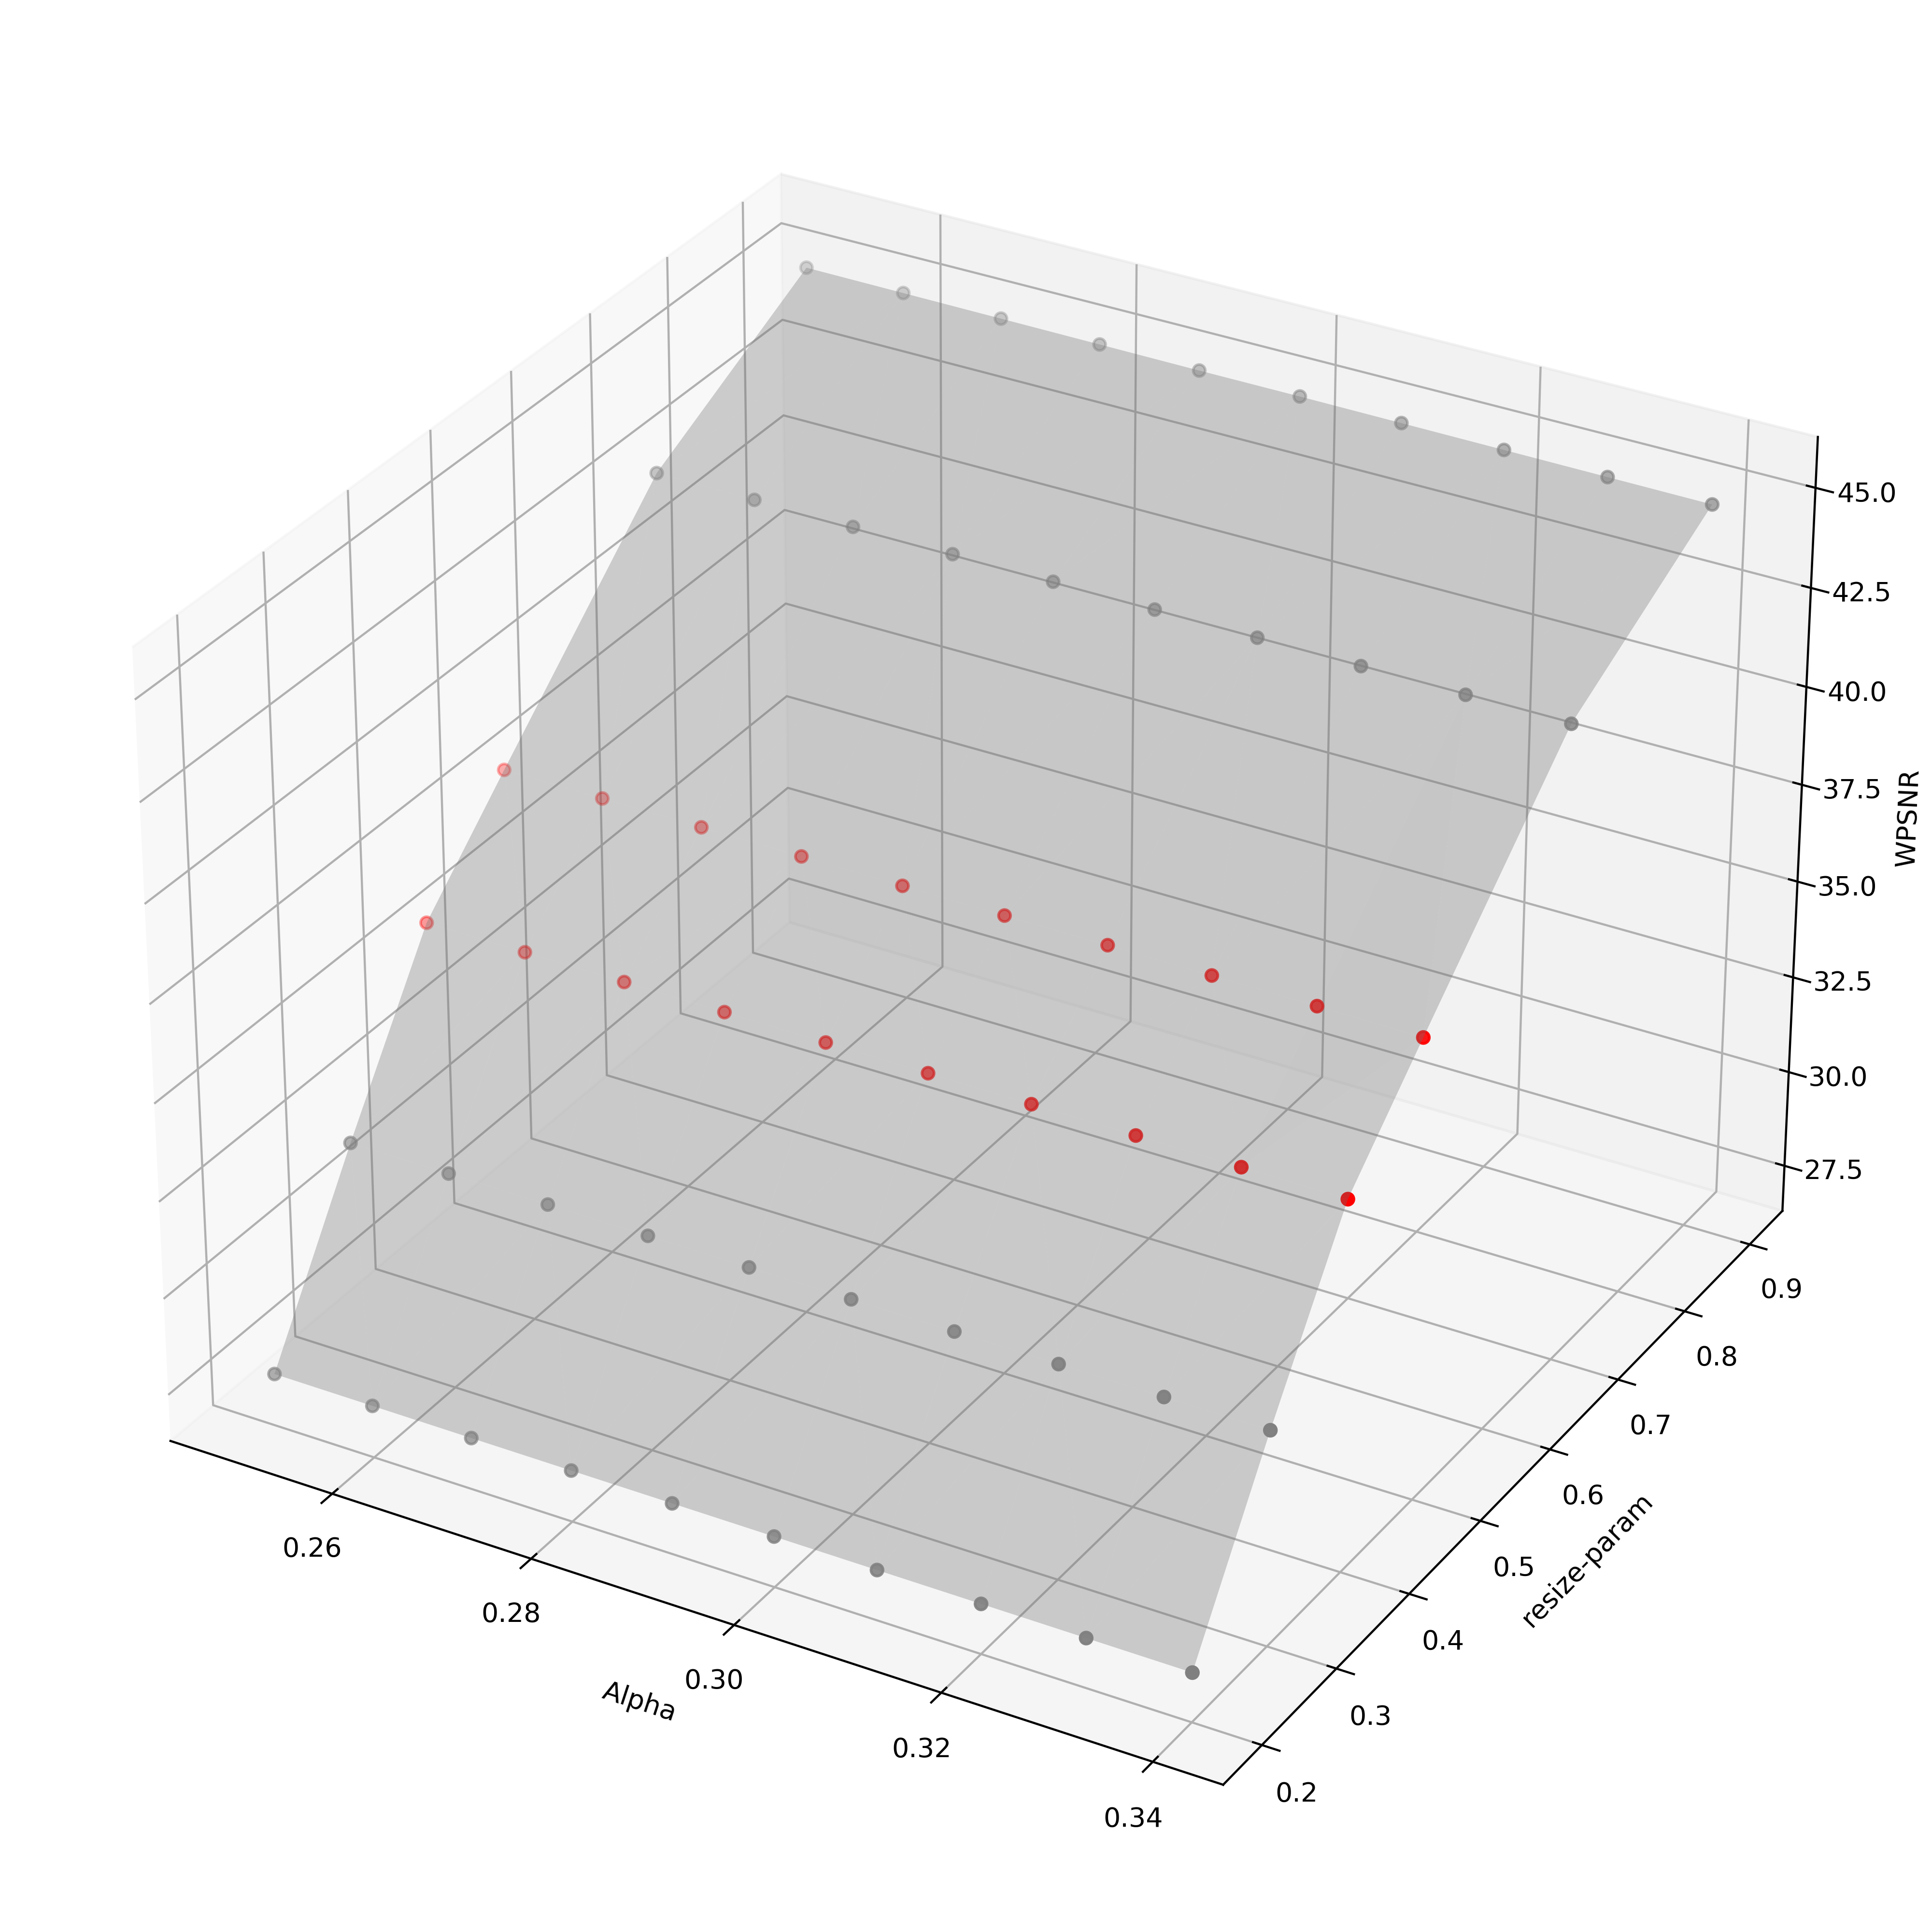
\includegraphics[width=0.5\textwidth]{../drawable/classic-attacks-plots/resize-alpha.png}
            \caption{Plot of $\alpha$, WPSNR and resize attacks. Red dots are successful attacks.}
        \end{figure}
    }

    \only<6>{
        \begin{figure}
            \centering
            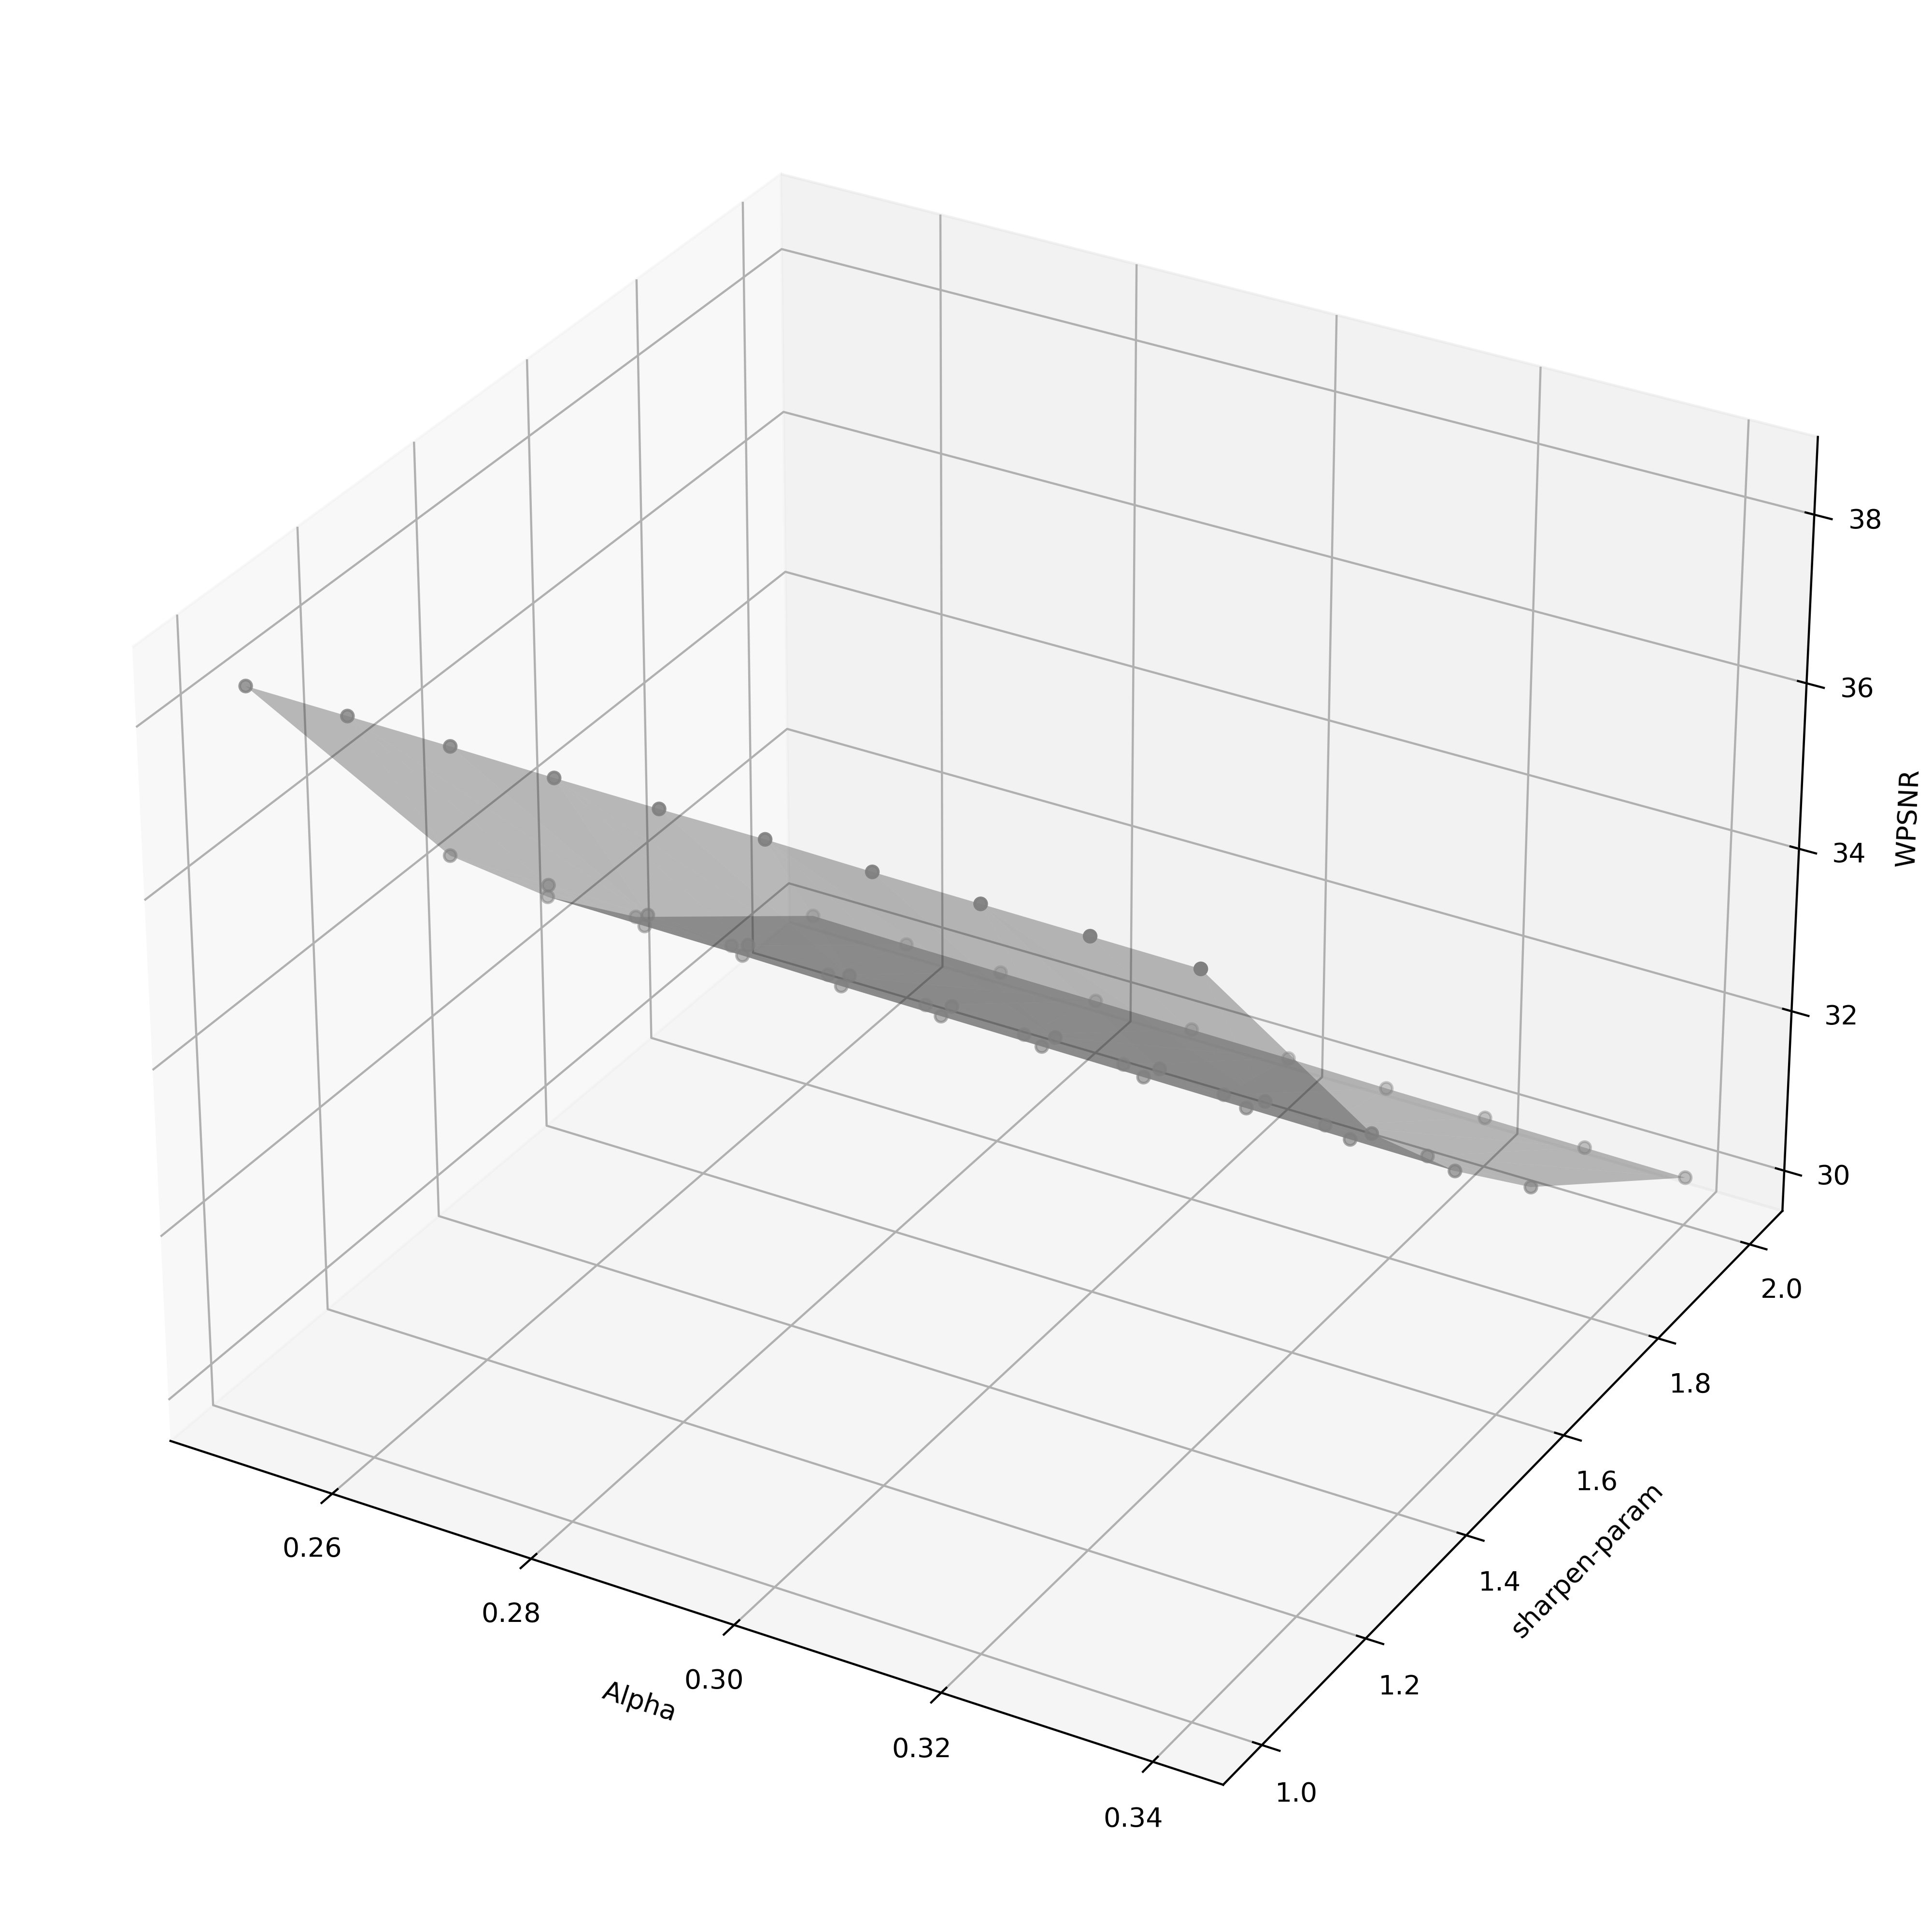
\includegraphics[width=0.5\textwidth]{../drawable/classic-attacks-plots/sharpen-alpha.png}
            \caption{Plot of $\alpha$, WPSNR and sharpen attacks (fixed sigma). Red dots are successful attacks.}
        \end{figure}
    }

\end{frame}

\subsection{Issues}
\begin{frame}
    \frametitle{Underflow/overflow problems}

    The underflows and overflows destroys parts of the mark during the embedding phase, resulting in information loss.

    \medskip

    \onslide<2->{
        A multitude of factors contributed to this game-losing, still-open issue:

        \medskip

        \begin{itemize}
            \item<3-> Bad typecasting in both embedding and detection caused conversion errors
            \item<4-> Editing a large number of coefficients in a small DCT and re-converting caused pixels to go negative or over 255

        \end{itemize}
    }

    \medskip

    \onslide<5->{
        During the re-conversion, the offending bits flipped and created white and dark patches in the image, razing the WPSNR and ruining the detection by up to 50/60\%.
    }
\end{frame}

\begin{frame}
    \frametitle{Underflow/overflow problems}

    We did not manage to fully fix the problem in time, and had to resort to approximations and a reduction in the $\alpha$ range for the day of the competition.

    \medskip

    \onslide<2->{
        Only a small subset $[ 0.4, 0.25 ]$ of the $\alpha$ managed to recover 100\% of the watermark without causing underflow/overflow problems. A range too low, that left us vulnerable to localized and resizing attacks.
    }

    \medskip

    \onslide<3->{
        With enough time, the problem could have been fixed by choosing a different DCT/pixel approach (e.g. working in the $-1/+1$ domain instead of the $0/255$ one)
    }

\end{frame}

\begin{frame}
    \frametitle{Possible improvements}

    What could be fixed or improved?

    \begin{itemize}
        \item<2-> Add heuristics to \texttt{texture\_areas} (e.g. randomizing the search, with a seed based on the hash of the image)
        \item<3-> Increase the block size $\Rightarrow 16 \times 16$
        \item<4-> Use machine learning to identify texture areas instead of metric-based deterministic function: CNN are great at finding patterns in images
        \item<5-> Employ smarter ways to optimize parameters instead of brute force
              % Altro?
    \end{itemize}
\end{frame}

\section{An aside: Wavelet embedding}

\begin{frame}
    \frametitle{Wavelet embedding}
    \onslide<1->{
        We experimented with wavelet embedding \footnote{Improved Wavelet-Based Watermarking Through Pixel-Wise Masking}.
        The embedding changes the coefficients on the HH and HL sub-band of the wavelets, where each coefficient gets the value:
        \[x_{ij}^* = x_{ij} + \alpha m_i\]
    }

    \onslide<2->{
        The extraction function is just the inverse of the embedding function.
        %ex_mark_value = (watermark_subband[r][c] - original_subband[r][c]) / alpha
        \[m_i = (x_{ij}^* - x_{ij}) / (x_{ij} \alpha ) \]
    }
\end{frame}

\begin{frame}
    \frametitle{Embedding and detection}

    \onslide<1>{
        Both procedures are quite simple.
    }

    \medskip

    \onslide<2->{
        For the embedding:
        \begin{enumerate}
            \item Extract DWT from image
            \item Embed contents of the mark into HL and HH subbands of the image
            \item Re-convert the image from DWT to pixel domain
        \end{enumerate}
    }

    \medskip

    \onslide<3->{
        For the detection:
        \begin{enumerate}
            \item Bring image into DWT domain
            \item Use inverse of embedding function to extract the mark components
        \end{enumerate}
    }

\end{frame}

\begin{frame}
    \frametitle{Mark visibility}
    Due to the simple implementation, the performance is not very good. The mark components are not weighted on the image contents, thus the mark is quite visible even with low $\alpha$ values (note "sawtooth pattern" on oblique lines).

    \medskip

    \begin{figure}[h]
        \centering
        \subfloat[]{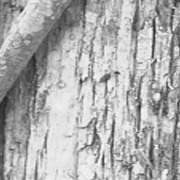
\includegraphics[width=0.34\textwidth]{../drawable/wavelets/original-detail.jpg}}  \quad
        \subfloat[]{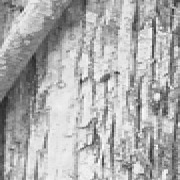
\includegraphics[width=0.34\textwidth]{../drawable/wavelets/wavelets-embedding-detail.jpg}}
        \caption{Detail of original (a) and watermarked image (b)}
        \label{fig:wavelet-watermark}
    \end{figure}
\end{frame}

\begin{frame}
    \frametitle{Performance}
    As expected by the simple embedding function, the defense against attacks is quite poor:
    \begin{figure}[h]
        \centering
        \subfloat[]{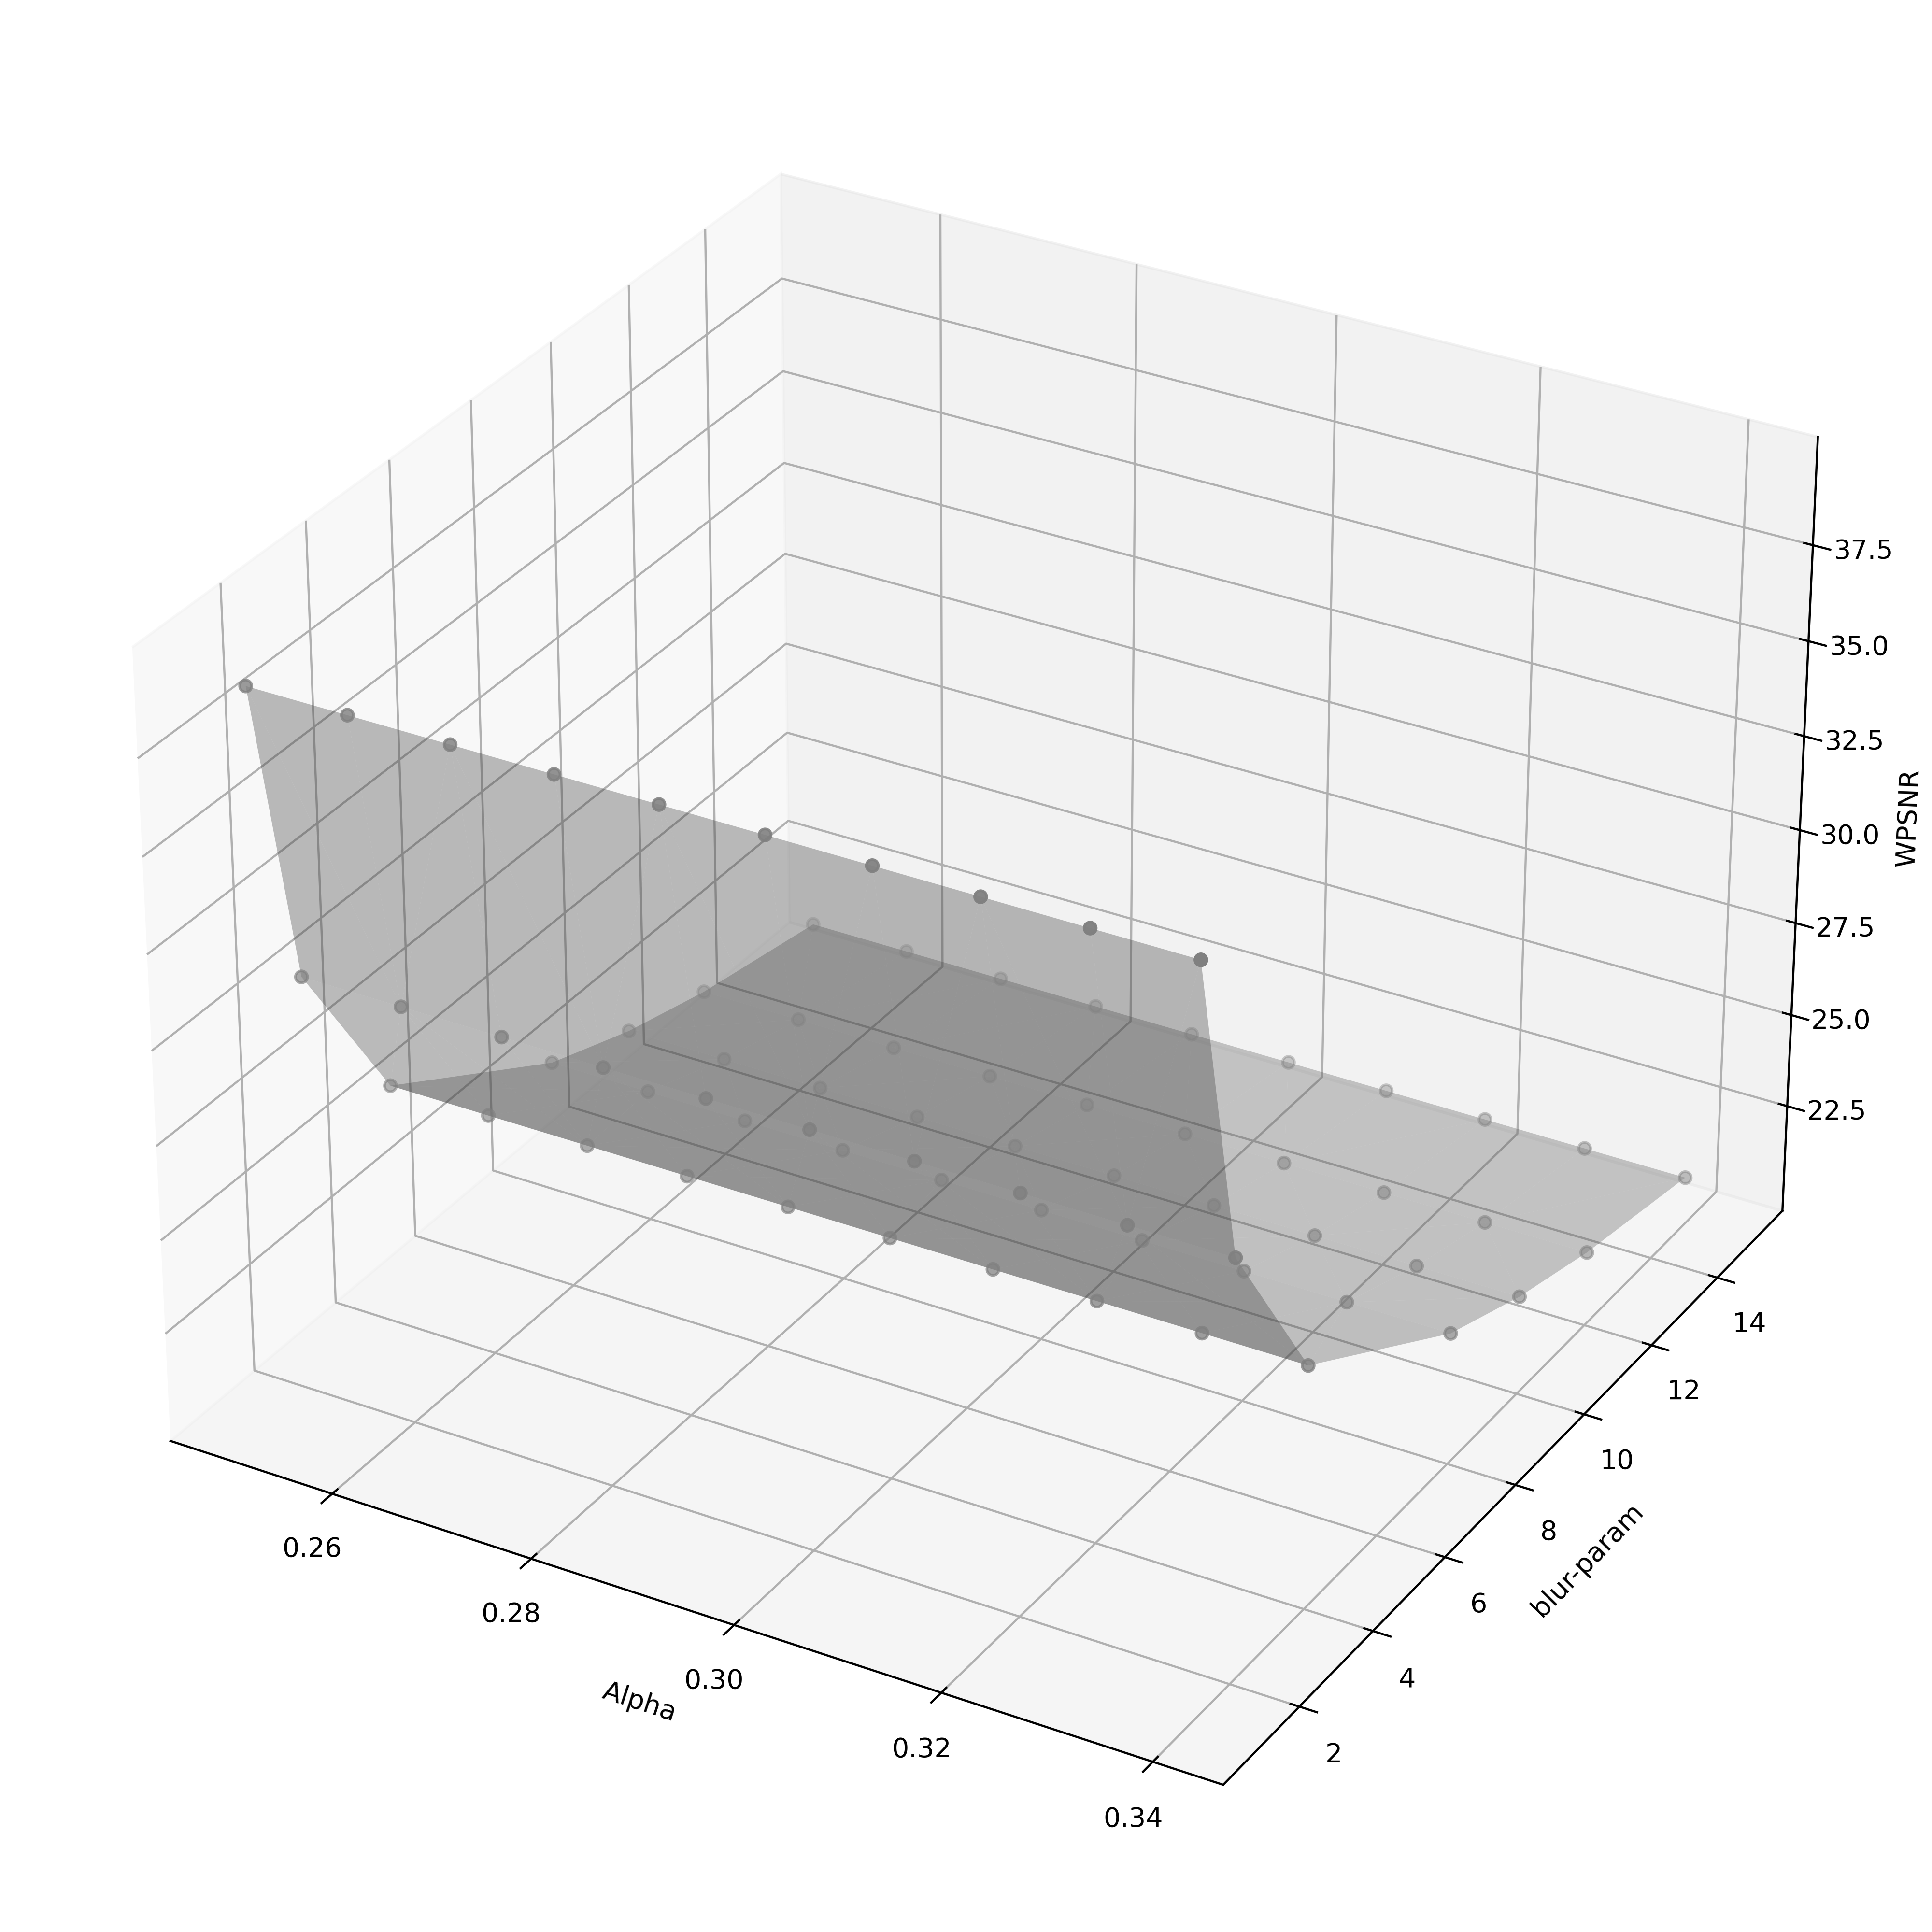
\includegraphics[width=0.34\textwidth]{../drawable/wavelets-attacks-plots/blur-alpha.png}}  \quad
        \subfloat[]{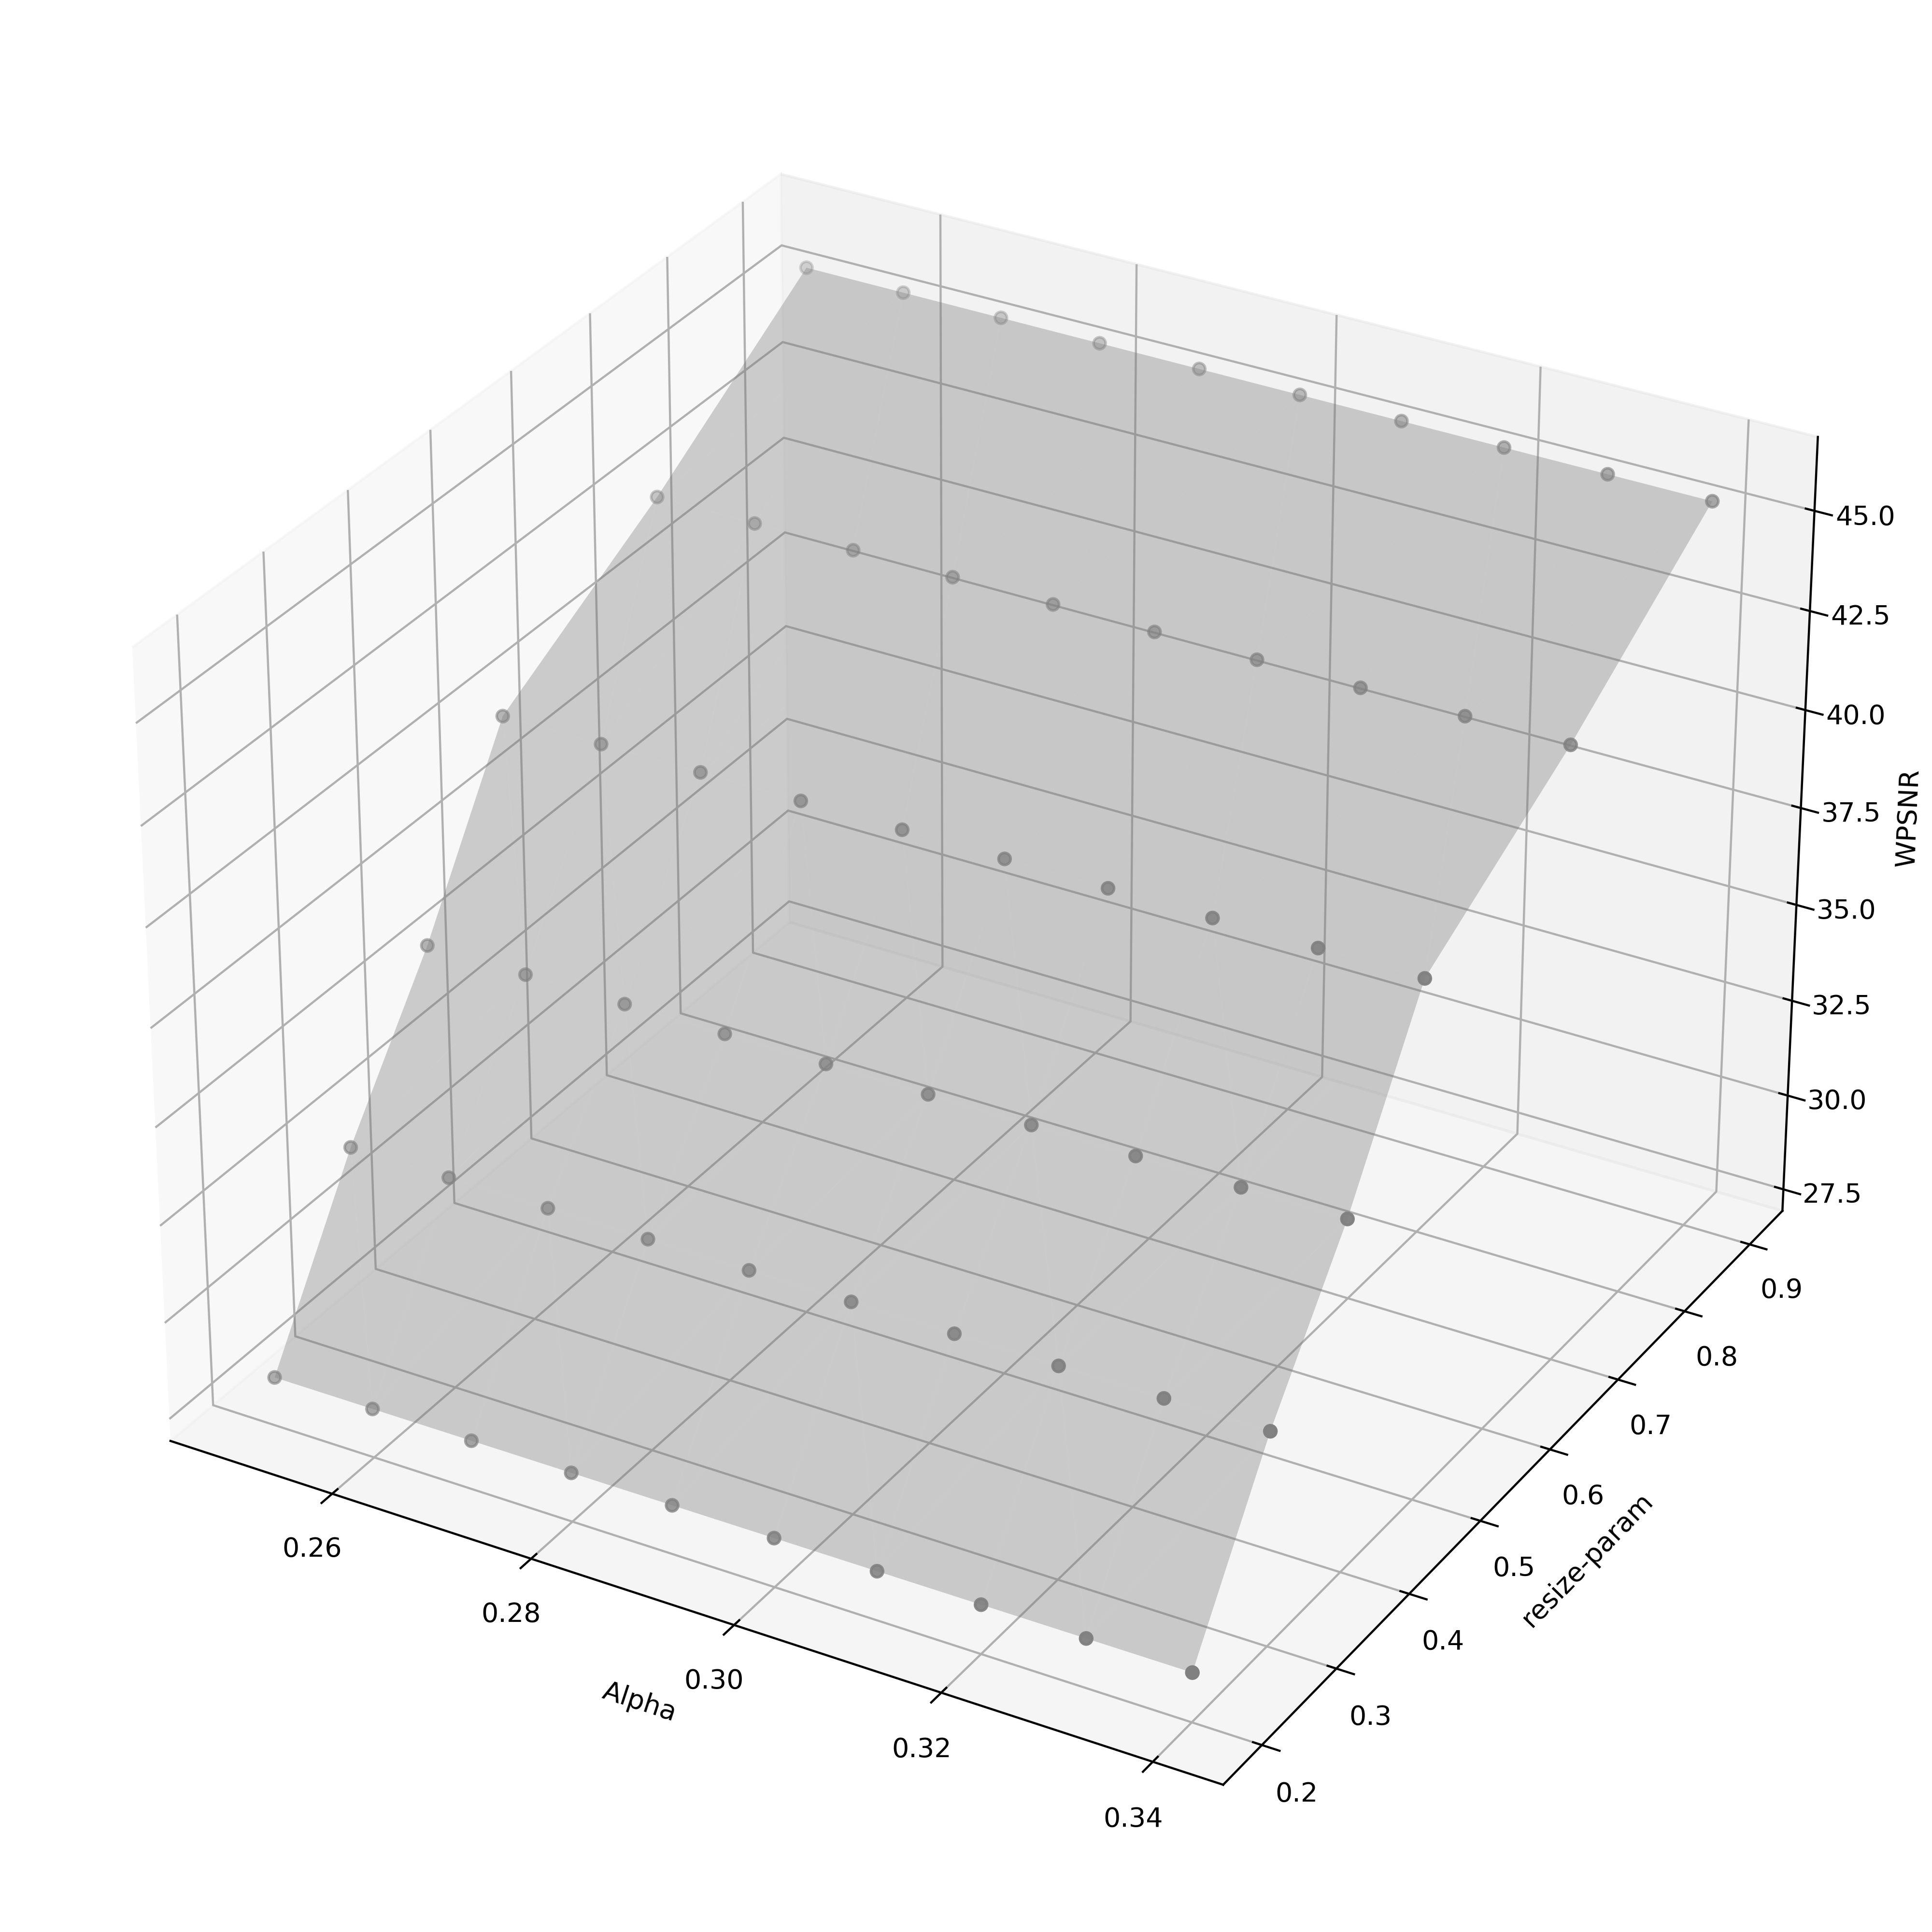
\includegraphics[width=0.34\textwidth]{../drawable/wavelets-attacks-plots/resize-alpha.png}}
        \caption{Plots of relation between WPSNR and attacks intensity}
        \label{fig:wavelet-performance-plots}
    \end{figure}
\end{frame}

\begin{frame}
    \frametitle{Conclusions}
    \onslide<1->{
        \begin{itemize}
            \item<1-> The mark is embedded with the same intensity on all components of the image, so is quite vulnerable to attacks and is visible even with low alphas
            \item<2-> Since we were short on time, we dropped this approach and kept the block-based embedding
        \end{itemize}
    }
\end{frame}

\section{Attack strategy}

\begin{frame}
    \frametitle{Attack strategy}
    We used a in-house interactive CLI program that mapped each \texttt{pyc} file to the each group image and allowed automated chain attacks.

    \begin{figure}
        \centering
        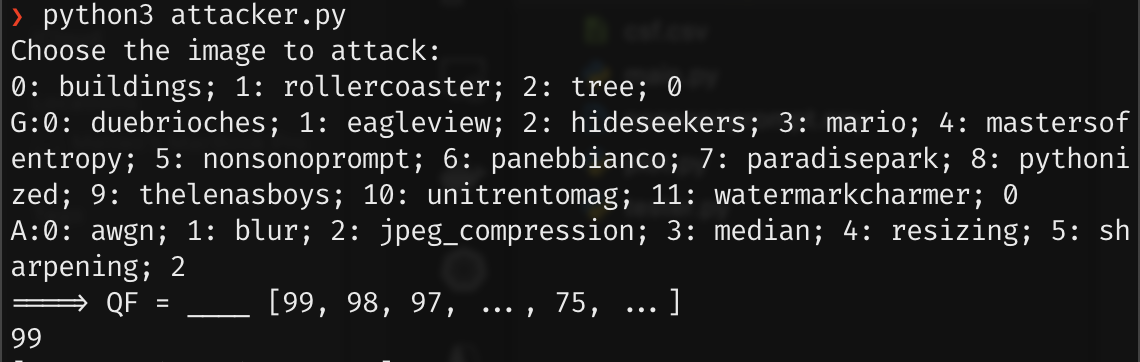
\includegraphics[width=\textwidth]{../drawable/attacker.png}
        \caption{A snippet of the attacker tool.}
    \end{figure}

\end{frame}

\begin{frame}
    \frametitle{Attack strategy}

    Some groups had very resistant watermarking, yet detectable by the eye.

    \onslide<2->{

        \begin{figure}[h]
            \centering
            \subfloat{
\includegraphics[width=.243\textwidth]{../drawable/bad1.png}} \quad
            \subfloat{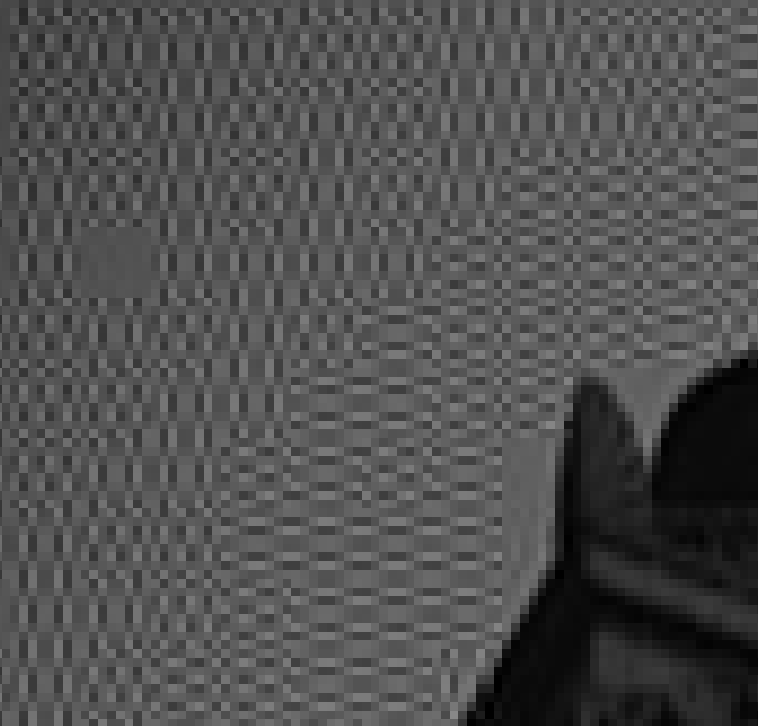
\includegraphics[width=.25\textwidth]{../drawable/bad2.png}}
            \caption{Example of very visible watermark implementations by groups \st{redacted} and \st{redacted}}
            \label{fig:blocks_rollecoaster_mark_visible}
        \end{figure}
    }

    \onslide<3->{
        These edge cases allowed us to narrow down possible attacks and focus on those who better affected that particular image (e.g. \texttt{median} for the right picture)
    }

\end{frame}

\begin{frame}
    \frametitle{Attack strategy}

    We managed to attack all groups in a rather short amount time, and this allowed to focus us on more resistant ones, in which we manually chained attacks and observed the behaviour in real-time in order to correct the strategy.

    \medskip

    \onslide<2-> {
        Interestingly enough, a number of pictures were easily destroyable with minimal amounts of resizing attacks (sometimes even scaling it by just 95\%)!
    }

    \medskip

    \onslide<3->{
        For some of the images maybe localized attacks were ideal: we did try them but with little to no success.
    }
\end{frame}

\section{Results}
\begin{frame}
    \frametitle{Results}
    \begin{itemize}
        \item \textbf{Invisibility}: visual quality of the image was neither excellent nor horrible; the final WPSNR achieve was in the $[50,60]$ range for all images
        \item<2-> \textbf{Activity}: we managed to successfully attack all groups, albeit with mediocre results
        \item<3-> \textbf{Robustness}: underflow/overflow problems were a pain in the neck, making us suffer on this side
        \item<4-> \textbf{Attack quality}: neither excellent nor horrible; some of the techniques were pretty easy to crack, while others were pretty hard
    \end{itemize}
\end{frame}